%!TeX root = BasiDiDati.tex

\chapter{Laboratorio}
PostgreSQL è un \textcolor{azzurrino}{\textbf{R}}elational \textcolor{azzurrino}{\textbf{D}}ata \textcolor{azzurrino}{\textbf{B}}ase \textcolor{azzurrino}{\textbf{M}}anagement \textcolor{azzurrino}{\textbf{S}}ystem con alcune funzionalità orientate agli oggetti.

L'interazione tra un utente (programmatore/utente finale) e le basi di dati gestite da PostgreSQL avviene secondo il modello client-server.

\begin{figure}[H]
  \centering
  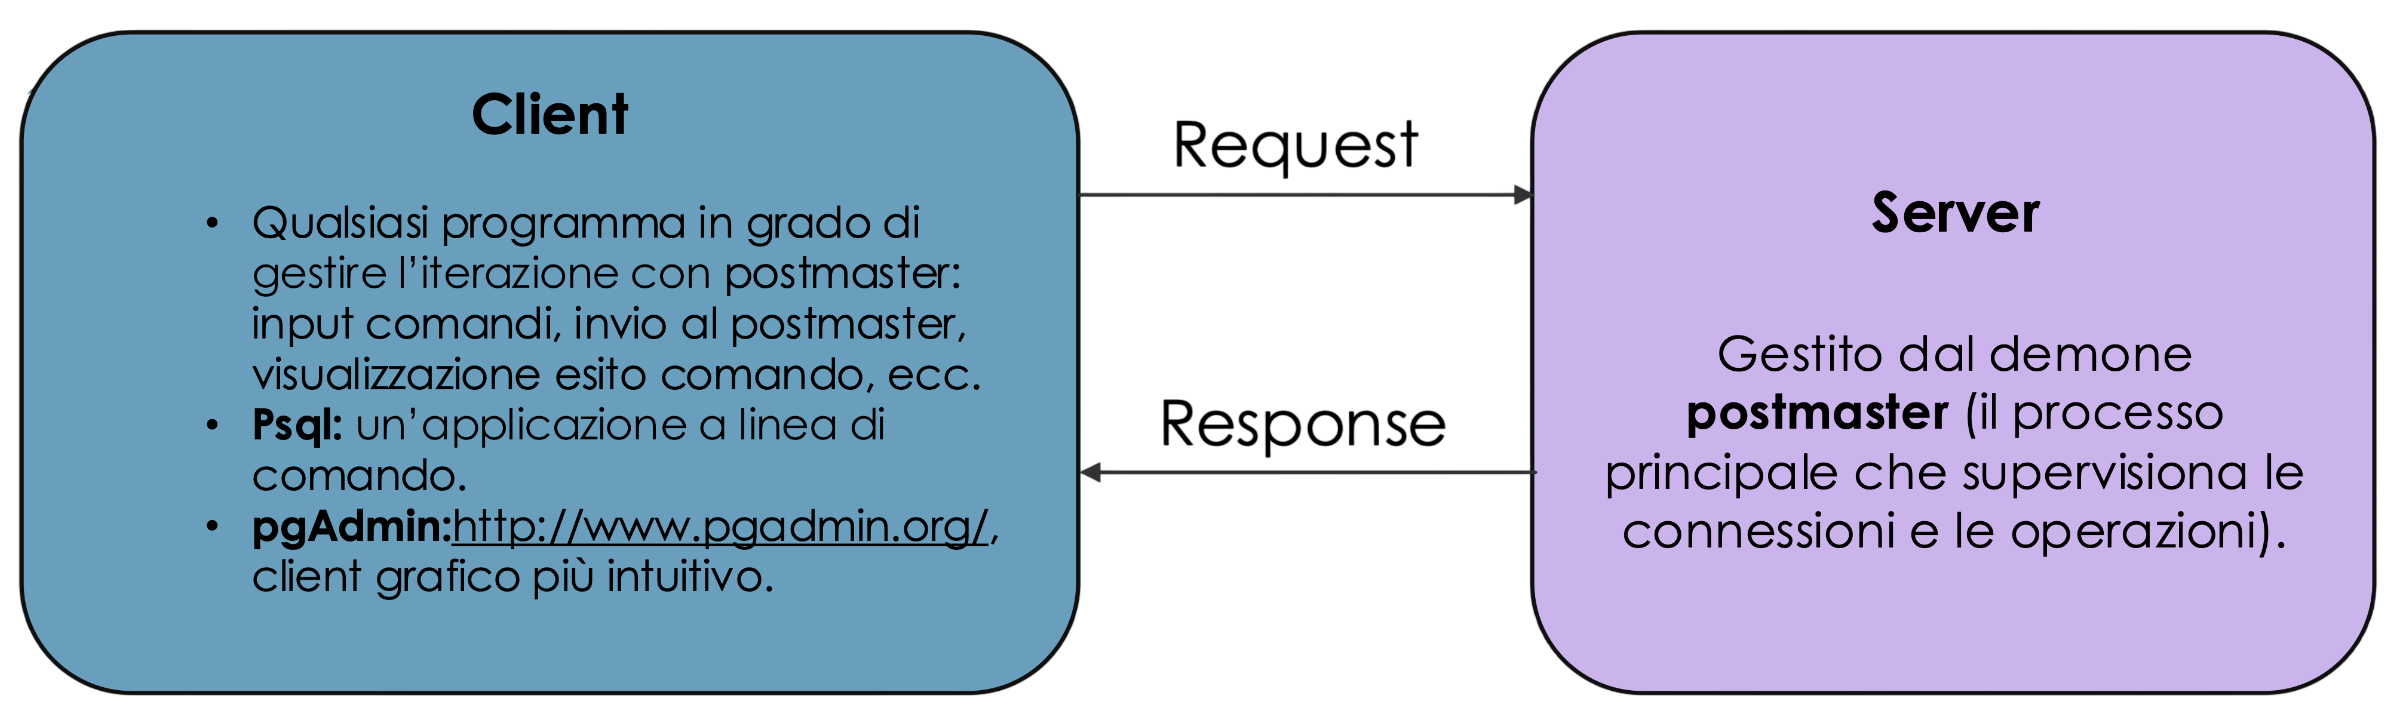
\includegraphics[width=0.8\textwidth]{images/ClientServer.png}
\end{figure}

\section{Comando \protect\texttt{CREATE TABLE}}
Il comando $\verb|CREATE TABLE|$ definisce uno schema di relazione e ne crea un'istanza vuota, specificando attributi, domini e vincoli.

La sintassi è:
\begin{codiceSQL}
CREATE TABLE tabella(
  attributo dominio [valoreDefault] {vincolo},
  attributo dominio [valoreDefault] {vincolo},
  {vincoloTabella}
);
\end{codiceSQL}

dove:
\begin{itemize}[label=$\triangleright$, itemsep=\smallskipamount]
  \item $\verb|[]|$: indicano parti opzionali
  \item $\verb|[valoreDefault]|$: indica un eventuale valore di default
  \item $\verb|{}|$: indica un elemento che può essere ripetuto 0 o più volte
  \item $\verb|{vincolo}|$: indica eventuali (0 o più) vincoli per ogni attributo
\end{itemize}

\begin{esempiobox}{Utilizzo di \texttt{CREATE TABLE}}
\begin{codiceSQL}
CREATE TABLE Impiegato (
  Matricola CHARACTER(6) PRIMARY KEY, 
  Nome VARCHAR(20) NOT NULL, 
  Cognome VARCHAR(20) NOT NULL,
  Dipart VARCHAR(15), 
  Stipendio NUMERIC(9) DEFAULT 0,
  FOREIGN KEY(Dipart) 
    REFERENCES Dipartimento(NomeDip),     -- vincolo di tabella
  UNIQUE (Cognome,Nome)                   -- vincolo di tabella
);
\end{codiceSQL}
\end{esempiobox}

\subsection{Identificatori}
\definizione{identificatore}{
  Un \textbf{identificatore} è una sequenza di caratteri che identifica un elemento del database (tabella, attributo, vincolo, ecc.).
}

Gli identificatori, in SQL, devono rispettare alcune regole:
\begin{itemize}[label=$\diamond$, itemsep=\smallskipamount]
  \item iniziare con una lettera (UTF-8) o un underscore (\_)
  \item possono contenere lettere, numeri (0-9) o underscore (\_)
  \item non possono essere parole chiave riservate a SQL
\end{itemize}

\vario{Nota}{
  Gli identificatori \textbf{non sono case sensitive}! (\texttt{idPersona} = \texttt{idpersona})
}

\subsection{Domini elementari}
\definizione{domini elementari}{
  I domini elementari (predefiniti) sono:
  \begin{itemize}[label=$\triangleright$, itemsep=\smallskipamount]
    \item \textbf{caratteri}: singoli caratteri o stringhe anche di lunghezza variabile
    \item \textbf{bit}: bit singoli (booleani) o stringhe di bit
    \item \textbf{numeri esatti e approssimati}
    \item \textbf{istanti temporali}
    \item \textbf{intervalli temporali}
  \end{itemize}
}

\subsubsection{Tipo carattere}
Permette di rappresentare singoli caratteri oppure stringhe.

Un carattere o stringa di caratteri sono rappresentati tra apici ('):
\texttt{'a'}, \texttt{'Questa è una stringa'}.

La sintassi è:
\begin{codiceSQL}
CHARACTER [VARYFING] [(lunghezza)]
\end{codiceSQL}

dove:
\begin{itemize}[label=$\triangleright$]
  \item $\verb|lunghezza|$: può essere fissa o variabile
  \begin{itemize}[label=$\diamond$, itemsep=\medskipamount]
    \item $\verb|CHARACTER|$: carattere singolo
    \item $\verb|CHARACTER(20)|$: stringa di lunghezza fissa (20 caratteri).
    
    Se la stringa è più corta di 20 caratteri, viene riempita con spazi a destra
    \item $\verb|CHARACTER VARYFING(20)|$ o $\verb|VARCHAR(20)|$: stringa di lunghezza variabile (max. 20 caratteri)
    \item $\verb|TEXT|$: stringa di lunghezza variabile senza limite fissato
  \end{itemize}
\end{itemize}

\subsubsection{Tipo boolean}
Permette di rappresentare valori booleani (\texttt{true} o \texttt{false}), più lo stato nullo.

La sintassi è:
\begin{codiceSQL}
BOOLEAN
\end{codiceSQL}

La rappresentazione dei valori booleani può essere:
\begin{itemize}[label=$\circ$, itemsep=\smallskipamount]
  \item $\verb|TRUE|$ o $\verb|FALSE|$
  \item $\verb|t|$ o $\verb|f|$
  \item $\verb|1|$ o $\verb|0|$
  \item $\verb|yes|$ o $\verb|no|$
  \item $\verb|NULL|$
\end{itemize}

\subsubsection{Tipo numerico esatto}
Permettono di rappresentare valori esatti (interi o con una parte decimale di lunghezza prefissata):
\begin{itemize}[label=$\triangleright$, itemsep=\medskipamount]
  \item \textbf{valori interi}:
  \begin{itemize}[label=$\diamond$, itemsep=\smallskipamount]
    \item $\verb|SMALLINT|$: valori interi (2 bytes: da -32.768 (215) a +32.767 (215-1))
    \item $\verb|INTEGER|$: valori interi (4 bytes: da -2147483648 (231) to +2147483647 (231-1))
  \end{itemize}
  \item \textbf{valori decimali}:
  \begin{itemize}[label=$\diamond$, itemsep=\smallskipamount]
    \item $\verb|NUMERIC [(precisione [, scala])]|$:
    \begin{itemize}[label=$\circ$, itemsep=\smallskipamount]
      \item $\verb|precisione|$: numero totale di cifre significative (cifre a sinistra e a destra della virgola)
      \item $\verb|scala|$: numero di cifre dopo la virgola (vuoto = 0)
    \end{itemize}
  \item $\verb|DECIMAL [(precisione [, scala])]|$: equivalente al precedente
  \end{itemize}
\end{itemize}

\esempio{tipo numerico esatto}{
  \texttt{NUMERIC(5,2)} permette di rappresentare valori come 100.01, 100.999 (arrotondato a 101.00), ma non valori come 1000.01
}

\subsubsection{Tipo numerico approssimato}
Permettono di rappresentare valori in virgola mobile:
\begin{itemize}[label=$\diamond$, itemsep=\smallskipamount]
  \item $\verb|REAL|$: precisione di 6 cifre decimali
  \item $\verb|DOUBLE PRECISION|$: precisione di 15 cifre decimali
\end{itemize}

\smallskip
Ciascun numero è rappresentato da una coppia di valori: \textbf{mantissa} (numero frazionario) + \textbf{esponente} (numero intero).\\[0.2ex]
Il valore si ottiene moltiplicando la mantissa per la potenza di 10 con grado pari all'esponente:
\begin{itemize}[itemsep=\smallskipamount]
  \item numero 0.17E16 corrisponde a $1,7 \times 10^{15}$
  \item numero -0.4E-6 corrisponde a $-4 \times 10^{-7}$
\end{itemize}

\subsubsection{Istanti temporali}
Permettono di rappresentare istanti di tempo.
\begin{itemize}[label=$\diamond$, itemsep=\medskipamount]
  \item $\verb|DATE|$: istanti del tipo (anno, mese, giorno)
  
  Si rappresenta tra apici (es. $\verb|'2025-12-01'|$) e lo standard ISO prescrive il formato \texttt{YYYY-MM-DD}
  \item $\verb|TIME [(precisione)][WITH TIME ZONE]|$: istanti del tipo (hour, minute, second)
  \begin{itemize}[itemsep=\smallskipamount]
    \item $\verb|precisione|$: numero cifre decimali per rappresentare frazioni del secondo
    \item $\verb|WITH TIME ZONE|$: permette di specificare anche [+-] hour: minute, che rappresentano la differenza con l'ora di Greenwich, o nomeFusoOrario
  \end{itemize}
  \item $\verb|TIMESTAMP [(precisione)][WITH TIME ZONE]|$: date + time
\end{itemize}

\subsubsection{Intervalli temporali}
Rappresenta un intervallo di tempo.

La sintassi è:
\begin{codiceSQL}
INTERVAL PrimaUnitaTempo [TO UltimaUNitaTempo]
\end{codiceSQL}

dove:
\begin{itemize}[label=$\triangleright$]
  \item $\verb|PrimaUnitàDiTempo|$ e $\verb|UltimaUnitàDiTempo|$: definiscono le unità di misura che devono essere utilizzate, dalla più precisa alla meno precisa
\end{itemize}

L'insieme delle unità di misura è diviso in due insiemi distinti:
\begin{itemize}
  \item Year-Month
  \item Day-Hour–Minute-Second
\end{itemize}

\subsection{Domini definiti dall'utente}
Per creare un dominio si esegue il comando:
\begin{codiceSQL}
CREATE DOMAIN nome AS tipoBase [valoreDefault][vincolo]
\end{codiceSQL}

dove:
\begin{itemize}[label=$\triangleright$]
  \item $\verb|CREATE DOMAIN|$: definisce un dominio, utilizzabile in definizioni di relazioni, anche con vincoli e valori di default
\end{itemize}

Il dominio può essere definito a partire da un dominio elementare oppure da un altro dominio definito dall'utente.

\begin{esempiobox}{Comando \texttt{CRETATE DOMAIN}}
\begin{codiceSQL}
CREATE DOMAIN giorniSettimana AS CHARACTER(3)
 CHECK(VALUE IN('LUN', 'MAR', 'MER', 'GIO', 'VEN', 'SAB', 'DOM'));

CREATE DOMAIN Voto AS SMALLINT DEFAULT NULL
 CHECK (value >= 18 AND value <= 30);
\end{codiceSQL}
\end{esempiobox}

\subsection{Vincoli intrarelazionali}
I vincoli intrarelazionali sono vincoli che si applicano a livello di relazione, cioè a una singola tabella.

I principali vincoli intrarelazionali sono:
\begin{itemize}[label=$\diamond$, itemsep=\medskipamount]
  \item $\verb|NOT NULL|$: valore nullo non è ammesso per l'attributo, quindi il valore deve sempre essere specificato, o si assegna un valore di default
  \item $\verb|UNIQUE|$: definisce (super)chiavi
\begin{codiceSQL}
Nome VARCHAR(20),
Cognome VARCHAR(20),
UNIQUE(Nome, Cognome)
--impone che non ci siano due righe che abbiano uguale
--sia il nome che il cognome
\end{codiceSQL}

\begin{codiceSQL}
Nome VARCHAR(20) UNIQUE,
Cognome VARCHAR(20) UNIQUE
--impone che non ci siano due righe che abbiano lo stesso nome
--o lo stesso cognome 
\end{codiceSQL}
  \item $\verb|PRIMARY KEY|$: chiave primaria (una sola, implica \texttt{NOT NULL}) 
\begin{codiceSQL}
matricola CHAR(6) PRIMARY KEY;
--se unico componente della chiave primaria
\end{codiceSQL}

\begin{codiceSQL}
nome VARCHAR(20),
cognome VARCHAR(20),
PRIMARY KEY(nome, cognome)
--se la chiave primaria ha piu' attributi
\end{codiceSQL}
  \item $\verb|CHECK|$: specifica un vincolo generico che deve soddisfare le tuple della tabella. 
  
  Viene soddisfatto se la sua espressione è vera o nulla
\begin{codiceSQL}
CREATE TABLE Impiegato(
matricola CHAR(6) PRIMARY KEY,
nome VARCHAR(20) NOT NULL,
cognome VARCHAR(20) NOT NULL,
qualifica VARCHAR(20),
stipendio NUMERIC(8,2) DEFAULT 500.00 NOT NULL
CHECK(stipendio >= 0.0),    --check di attributo
UNIQUE(cognome, nome),
CHECK(nome <> cognome)      --check di tabella
)
\end{codiceSQL}
\end{itemize}

\subsection{Vincoli interrelazionali}
Un vincolo di integrità referenziale (interrelazionale) crea un legame tra i valori di un attributo (o di un insieme di attributi) A della tabella corrente (interna/slave) e i valori di un attributo (o di un insieme di attributi) B di un'altra tabella (esterna/master).

\smallskip
Il vincolo impone che:
\begin{itemize}[label=$\diamond$, itemsep=\smallskipamount]
  \item in ogni tupla della tabella interna, il valore di A, se diverso dal valore nullo, sia presente tra i valori di B nella tabella esterna
  \item  l'attributo B della tabella esterna deve essere soggetto a un vincolo \texttt{UNIQUE} (o \texttt{PRIMARY KEY})
\end{itemize}

\vario{Nota}{
  L'attributo (o insieme di attributi) B può anche non essere la chiave primaria, ma deve essere identificante per le tuple della tabella esterna.
}

\hl{\texttt{REFERENCES} e \texttt{FOREIGN KEY} permettono di definire vincoli di integrità referenziale}.

Per singoli attributi basta utilizzare il costrutto \texttt{REFERENCES}.
\begin{codiceSQL}
CREATE TABLE Impiegato (
  Matricola CHARACTER(6) PRIMARY KEY,
  Nome CHARACTER VARYING(20) NOT NULL,
  Cognome CHARACTER VARYING(20) NOT NULL,
  Dipart CHARACTER VARYING(15),
    REFERENCES Dipartimento(NomeDip),  --attributo chiave (singolo) di tabella esterna
  Ufficio NUMERIC(3),
  Stipendio NUMERIC(9) DEFAULT 0,
  UNIQUE(Cognome, Nome)
)
\end{codiceSQL}

Per attributi multipli, si usa il costrutto \texttt{FOREIGN KEY} alla fine della definizione degli attributi, seguito da \texttt{REFERENCES}.
\begin{codiceSQL}
CREATE TABLE Impiegato (
  Matricola CHARACTER(6) PRIMARY KEY,
  Nome CHARACTER VARYING(20) NOT NULL,
  Cognome CHARACTER VARYING(20) NOT NULL,
  Dipart CHARACTER VARYING(15),
  REFERENCES Dipartimento(NomeDip),   
  Ufficio NUMERIC(3),
  Stipendio  NUMERIC(9) default 0,
  FOREIGN KEY(Nome, Cognome)
    REFERENCES Anagrafica (Nome, Cognome) --tabella esterna con attributi chiave
)
\end{codiceSQL}

\smallskip
Vediamo un esempio più concreto:

\begin{figure}[H]
  \centering
  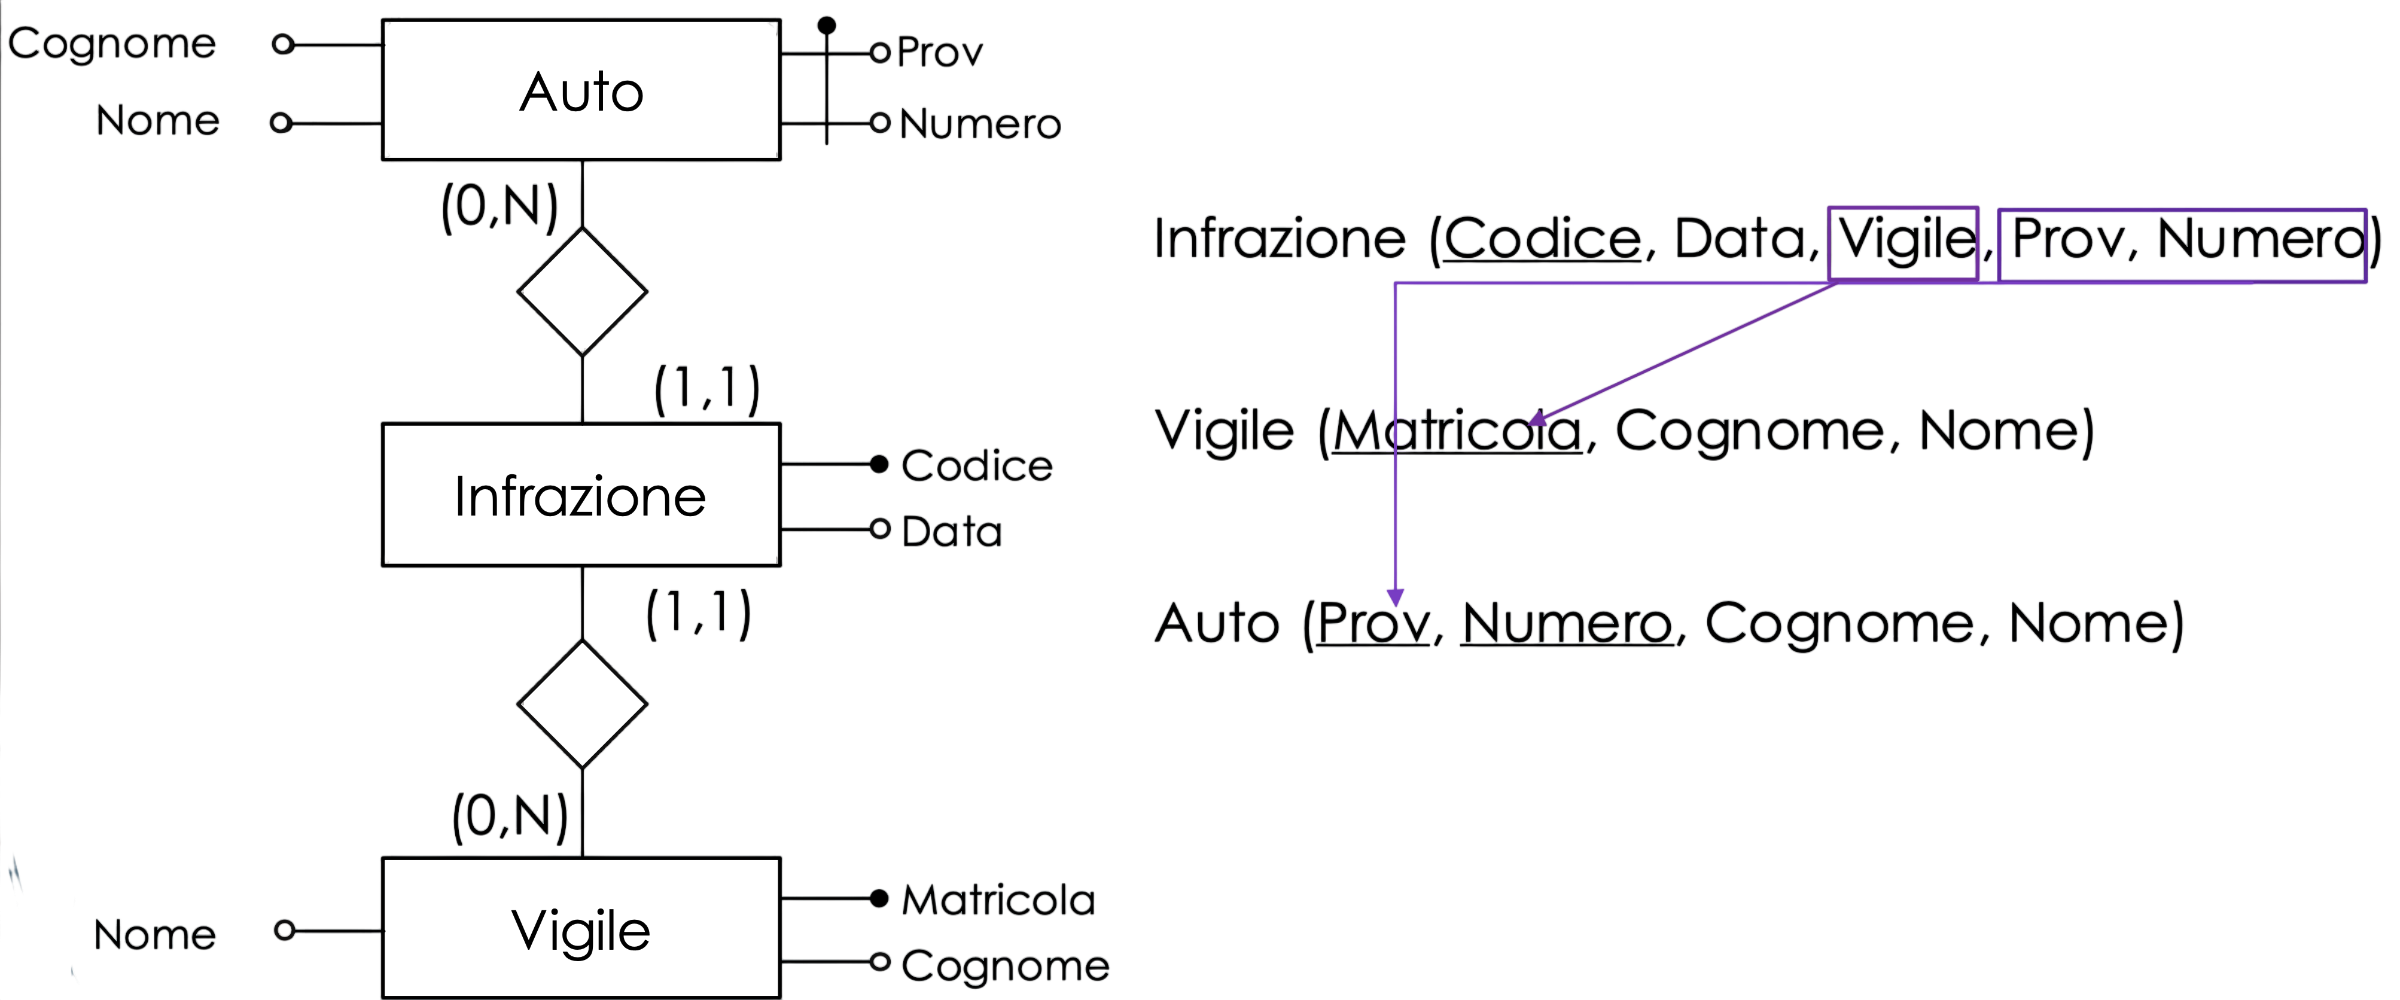
\includegraphics[width=0.7\textwidth]{images/esempioReferences.png}
\end{figure}

\begin{codiceSQL}
CREATE TABLE Infrazione(
  Codice CHAR(6) PRIMARY KEY, 
  Data DATE NOT NULL,  
  Vigile INTEGER NOT NULL
  REFERENCES Vigile(Matricola),
  Provincia CHAR(2),  
  Numero CHAR(6) ,
  FOREIGN KEY(Provincia, Numero)
    REFERENCES Auto(Provincia, Numero)
)
\end{codiceSQL}

\section{Modifica degli schemi}
\begin{itemize}[label=$\triangleright$, itemsep=\smallskipamount]
  \item \texttt{ALTER}: effettua modifiche (a domini, tabelle...), ad esempio aggiungere una colonna a una relazione
  \item \texttt{DROP DOMAIN}: permette di rimuovere i domini
  \item \texttt{DROP TABLE}: cancella una tabella
\end{itemize}

\subsection{Comando \texttt{ALTER TABLE}}
Il costrutto \texttt{ALTER} permette di:
\begin{itemize}[label=$\circ$, itemsep=\medskipamount]
  \item \textbf{aggiungere un nuovo attributo} (\texttt{ADD COLUMN}):
\begin{codiceSQL}
ALTER TABLE tabella
ADD COLUMN attributo tipo;

ALTER TABLE impiegato
ADD COLUMN stipendio NUMERIC(8,2);
\end{codiceSQL}
  \item \textbf{rimuovere un attributo} (\texttt{DROP COLUMN}):
\begin{codiceSQL}
ALTER TABLE tabella
DROP COLUMN attributo;

ALTER TABLE impiegato
DROP COLUMN stipendio;
\end{codiceSQL}
  \item \textbf{modificare valore di default di un attributo} (\texttt{ALTER COLUMN}):
\begin{codiceSQL}
ALTER TABLE tabella 
ALTER COLUMN attributo { SET DEFAULT valore | DROP DEFAULT };

ALTER TABLE impiegato 
ALTER COLUMN stipendio SET DEFAULT 1000.00;
\end{codiceSQL}
\end{itemize}

\section{Comando \texttt{DELETE} e \texttt{DROP TABLE}}
Le tuple di una tabella vengono cancellate con il comando \texttt{DELETE}:
\begin{codiceSQL}
DELETE FROM tabella [ WHERE condizione ];
\end{codiceSQL}

dove:
\begin{itemize}[label=$\triangleright$, itemsep=\smallskipamount]
  \item \texttt{condizione}: espressione booleana che seleziona quali tuple cancellare
\end{itemize}

\vario{Nota}{
  Se non viene specificata la condizione \texttt{WHERE}, verrano cancellate tutte le tuple.
}
\begin{codiceSQL}
DELETE FROM impiegato WHERE matricola = 'A001';
\end{codiceSQL}

\bigskip
Una tabella viene cancellata con il comando \texttt{DROP TABLE}:
\begin{codiceSQL}
  DROP TABLE tabella;
\end{codiceSQL}

\section{Comando \texttt{INSERT INTO} e \texttt{UPDATE}}
Il comando \texttt{INSERT INTO} permette di inserire valori all'interno di una tupla:
\begin{codiceSQL}
INSERT INTO Tabella [ ( Attributi ) ] 
VALUES( Valori )

--oppure

INSERT INTO Tabella [ ( Attributi )]
(SELECT ...)
\end{codiceSQL}

\begin{esempiobox}{Utilizzo di \texttt{INSERT INTO}}
\begin{codiceSQL}
INSERT INTO Museo(nome, citta, indirizzo, numeroTelefono, giornoChiusura, prezzo)
VALUES('Arena', 'Verona', 'piazza Bra', '045 8003204', 'MARTEDI', 20);
\end{codiceSQL}
\end{esempiobox}

\bigskip
Il comando \texttt{UPDATE} permette di aggiornare i valori all'interno di una tupla:
\begin{codiceSQL}
UPDATE NomeTabella
SET Attributo = < Espressione | SELECT ... | NULL | DEFAULT >
[ WHERE Condizione ]
\end{codiceSQL}

\begin{esempiobox}{Utilizzo di \texttt{INSERT INTO}}
\begin{codiceSQL}
UPDATE Museo SET sitoInternet = 'www.ciao.it' 
WHERE citta = 'Verona';  
\end{codiceSQL}
\end{esempiobox}


\section{Selezione}
La struttura base del comando di selezione è:
\begin{codiceSQL}
SELECT [ DISTINCT ]
[ * | expression [[ AS] output_name ] [, 
...] ]
FROM from_item [, ...] 
  [ WHERE condition ]
    [ GROUP BY grouping_element [, ...] ]
      [ HAVING condition [, ...] ]
      [ { UNION | INTERSECT | EXCEPT } [ DISTINCT
      ] other_select ]
        [ ORDER BY expression [ ASC | DESC | USING 
        operator ]]
\end{codiceSQL}


\subsection{Clausola \texttt{SELECT}}
\begin{codiceSQL}
SELECT [ DISTINCT ]
[{* | expression [[ AS] output_name ]} [, ...]]
\end{codiceSQL}

dove:
\begin{itemize}[label=$\triangleright$, itemsep=\smallskipamount]
  \item \texttt{*}: abbreviazione per indicare tutti gli attributi delle tabelle
  \item \texttt{expression}: espressione che coinvolge gli attributi della tabella (può anche essere semplicemente il nome di un attributo)
  \item \texttt{output\_name}: nome assegnato all’attributo che conterrà il risultato della valutazione dell’espressione expression nella relazione risultato.
  \item \texttt{DISTINCT}: se presente richiede l’eliminazione delle tuple duplicate
\end{itemize}

\smallskip
L’esecuzione di una \texttt{SELECT} produce una relazione che:
\begin{itemize}[label=$\circ$, itemsep=\smallskipamount]
  \item ha come schema tutti gli attributi elencati nella clausola \texttt{SELECT}
  \item ha come contenuto tutte le tuple ottenute proiettando sugli attributi indicati nella \texttt{SELECT} provenienti dalle tabelle del \texttt{FROM} (prodotto cartesiano), limitate a quelle che soddisfano le eventuali condizioni specificate nelle clausole \texttt{WHERE}, \texttt{GROUP BY} e \texttt{HAVING}
\end{itemize}

\subsubsection{Target List}

\begin{minipage}[t]{0.39\textwidth}
   \begin{codiceSQL}
SELECT *
FROM Tabella
   \end{codiceSQL}
\end{minipage}
\hfill % Questo comando inserisce uno spazio flessibile che spinge le due minipage ai lati opposti
\begin{minipage}[t]{0.50\textwidth}
  \vspace{1em}
   Selezione di tutti gli attributi 
delle tabelle indicate nella 
clausola FROM
\end{minipage}

\begin{minipage}[t]{0.39\textwidth}
   \begin{codiceSQL}
SELECT Attributo1, Attributo2
FROM Tabella
   \end{codiceSQL}
\end{minipage}
\hfill % Questo comando inserisce uno spazio flessibile che spinge le due minipage ai lati opposti
\begin{minipage}[t]{0.50\textwidth}
  \vspace{1em}
   Selezione di tutti gli attributi 
delle tabelle indicate nella 
clausola FROM
\end{minipage}

\begin{esempiobox}{Esempio}
\begin{codiceSQL}
SELECT Nome, Reddito
FROM Persone
  WHERE Eta < 30;
\end{codiceSQL}

  \begin{figure}[H]
    \centering
    \includegraphics[width=0.6\textwidth]{images/nomeReddito.png}
    \caption{selezione solo delle tuple dove è rispettata la condizione}
  \end{figure}
\end{esempiobox}


\subsubsection{Concatenazione stringhe}
L'operatore di concatenazione \texttt{||} è un operatore scalare (o operatore di riga).

Lavora su una singola riga alla volta.\\[0.2ex]
Se la tua tabella ha 100 righe, il costrutto \texttt{SELECT titolo || ' - ' || città} calcolerà e restituirà 100 risultati testuali separati, uno per ogni riga.

\vario{Nota}{
  Non è un'esclusiva di \texttt{SELECT}, può infatti essere utilizzato anche nella clausola \texttt{WHERE} e nella clausola \texttt{ORDER BY}.
}

\smallskip
La concatenazione all'interno della clausola \texttt{WHERE} serve per filtrare i dati:
\begin{codiceSQL}
WHERE nome || ' ' || cognome = 'Mario Rossi'
--Trova la riga in cui l'unione di nome e cognome da esattamente 
--'Mario Rossi'
\end{codiceSQL}

\smallskip
La concatenazione all'interno della clausola \texttt{ORDER BY} serve per ordinare i risultati:
\begin{codiceSQL}
ORDER BY titolo || citta
--Ordina i risultati basandosi sull'unione testuale dei due campi
\end{codiceSQL}


\subsection{Clausola FROM}
\begin{codiceSQL}
FROM from_item [, ...]
\end{codiceSQL}

dove:
\begin{enumerate}[itemsep=\smallskipamount]
  \item  \texttt{table\_name [[AS] alias [(column\_alias [, ...])]]}
  \begin{itemize}[itemsep=\smallskipamount]
    \item se sono presenti due o più tabelle, si esegue il prodotto cartesiano tra tutte le  tabelle
    \item se ci sono attributi con lo stesso nome su tabelle diverse, nel \texttt{SELECT} questi attributi sono identificati anteponendo il nome della tabella e un \texttt{’.’}:  \texttt{nomeTabella.nomeAttributo}
  \end{itemize}

  \item  (other\_select) [AS] nomeRisultato [(column\_alias [,...])
  \begin{itemize}
    \item  è una SELECT innestata. Il risultato della SELECT interna è lo schema con nome 
nomeRisultato su cui fare la SELECT corrente.
  \end{itemize}

  \item  from\_item [NATURAL] join\_type from\_item [ON condition]
  \begin{itemize}
    \item  è la clausola JOIN.
    \item Metodo più sofisticato di 1) che permette di selezionare un sottoinsieme del 
prodotto cartesiano di due o più tabelle. join\_type specifica il tipo di join. I tipi 
principali sono riassunti nelle slide seguenti
  \end{itemize}
\end{enumerate}


\subsubsection{Uso di alias}

\begin{codiceSQL}
SELECT P.Reddito, R.Telefono
FROM Reparti as R, Persona ad P
WHERE ... ;
\end{codiceSQL}

Utile quando è necessario specificare la provenienza dell’attributo, 
perchè nella base di dati sono presenti più attributi con lo stesso nome

\subsubsection{Target List}
\begin{codiceSQL}
SELECT P.Nome as NPersona, P.Reddito as RPersona
FROM Persone as P
WHERE P.Eta < 30
\end{codiceSQL}




\subsection{Clausola WHERE}
\begin{codiceSQL}
  WHERE condition
\end{codiceSQL}

\textbf{\textcolor{black!50!red}{condition}} è un’espressione booleana combinando condizioni semplici $C_{i}$ con gli 
operatori AND, OR, NOT.
\begin{enumerate}
  \item  $C_{i}$ := expr [ $\theta$ \{expr | const\}]
dove
\begin{itemize}
  \item expr := espressione che contiene riferimenti agli attributi delle tabelle che compaiono 
nella clausola FROM.
\item $\theta \in$ \{=,<>,<,>,<=,>=\}
\item const := valore dei domini di base.
\end{itemize}
\item Una riga soddisfa \textcolor{black!50!red}{condition} se l’espressione è vera quando valutata con i valori 
della riga.
\item Una riga che non soddisfa condition è scartata dal risultato finale
\end{enumerate}





\begin{minipage}[t]{0.39\textwidth}
 \begin{codiceSQL}
SELECT Nome, Reddito
FROM Persone
WHERE Eta < 30;
\end{codiceSQL}
\end{minipage}
\hfill % Questo comando inserisce uno spazio flessibile che spinge le due minipage ai lati opposti
\begin{minipage}[t]{0.50\textwidth}
SELECT Nome, Reddito
FROM Persone
WHERE Età < 30 OR Reddito > 50;
\end{minipage}




\subsubsection{Operatore LIKE}
\begin{codiceSQL}
WHERE attributo [NOT] LIKE 'pattern';
\end{codiceSQL}

Nella clausola WHERE può apparire l’operatore LIKE per il confronto di stringhe. 
LIKE è un operatore di pattern matching. I pattern si costruiscono con i 
caratteri speciali \_ e \%:
\begin{itemize}
  \item \_ = 1 carattere qualsiasi.
  \item \% = 0 o più caratteri qualsiasi.
\end{itemize}


\begin{minipage}[t]{0.39\textwidth}
  \vspace{2em}
  \begin{codiceSQL}
SELECT Nome,Reddito
FROM Persona
WHERE Nome LIKE 'A\%a'
  \end{codiceSQL}
\end{minipage}
\hfill 
\begin{minipage}[t]{0.50\textwidth}
  \vspace{0pt}
  % Rimosso totalmente \begin{figure}[H] e \end{figure}
  \includegraphics[width=0.8\textwidth]{images/nomeReddito2.png}
\end{minipage}  


\subsubsection{Operatore SIMILAR TO}


L’operatore \textbf{\textcolor{purple}{SIMILAR TO}} è un \textbf{\textcolor{purple}{LIKE}} più espressivo che accetta, come pattern, 
un sottoinsieme delle espressioni regolari POSIX (versione SQL). 
Esempi di componenti di espressioni regolari:
\begin{itemize}
  \item \_ = 1 carattere qualsiasi. 
  \item \% = 0 o più caratteri qualsiasi.
  \item * = ripetizione del precedente match 0 o più volte.
  \item + = ripetizione del precedente match UNA o più volte.
  \item \{n,m\} = ripetizione del precedente match almeno n e non più di m volte.
  \item {[} ... {]} = ... è un elenco di caratteri ammissibili
\end{itemize}


\begin{minipage}[t]{0.50\textwidth}
  \vspace*{0pt}
  \begin{codiceSQL}[unbreakable]
SELECT *
FROM Persone
WHERE Nome SIMILAR TO '[AFO]'
  \end{codiceSQL}
\end{minipage}
\hfill 
\begin{minipage}[t]{0.45\textwidth}
  \vspace*{0pt}
  \vspace{1.5em} % Spazio per allineare il testo al centro del codice
Per trovare nomi che inziano per A,F o O
\end{minipage}  


\subsubsection{Operatore BETWEEN}

\begin{codiceSQL}
WHERE attributo [NOT] BETWEEN valore_iniziale AND valore_finale;
\end{codiceSQL}

Nella clausola \textcolor{purple}{\textbf{WHERE}} può apparire l’operatore \textcolor{purple}{\textbf{BETWEEN}} per testare l’appartenenza 
di un valore ad un intervallo (non limitato ai valori numerici, usato anche con date e 
stringhe)


\begin{minipage}[t]{0.40\textwidth}
  \begin{codiceSQL} 
SELECT *
FROM Persone
WHERE Eta BETWEEN 20 AND 40
  \end{codiceSQL}
\end{minipage}
\hfill 
\begin{minipage}[t]{0.45\textwidth}
  \includegraphics[width=0.8\textwidth, valign=t]{images/nomeEtaReddito.png}
\end{minipage}


\subsubsection{Operatore IN}
\begin{codiceSQL}
  WHERE attributo [NOT] IN ( valore [, ...] );

\end{codiceSQL}
Nella clausola WHERE può apparire l’operatore [\textbf{\textcolor{purple}{NOT}}] \textbf{\textcolor{purple}{IN}} per testare 
l’appartenenza di un valore ad un insieme.
\begin{codiceSQL}
SELECT *
FROM Persone
WHERE Nome NOT IN ('Andrea', 'Franco')
\end{codiceSQL}

\subsubsection{Operatore IS NULL}
\begin{codiceSQL}
WHERE attributo IS [ NOT ] NULL;
\end{codiceSQL}
Nella clausola WHERE può apparire l’operatore \textbf{\textcolor{purple}{IS}} [\textbf{\textcolor{purple}{NOT}}] \textbf{\textcolor{purple}{NULL}} per testare se un 
valore è \textbf{\textcolor{purple}{NOT KNOWN (NULL)}} o no.
Il valore NULL non rappresenta lo zero o una stringa vuota, ma l'assenza di dati 
o un valore sconosciuto.
A partire dalle versioni SQL-2 è stata adottata una logica a tre valori (true, 
false, unknown) e i valori nulli non sono considerati né veri, né falsi.\par
\begin{center}
NON SI PUÒ usare ’=’ o ’<>’ con il valore NULL!  
\end{center}

\begin{codiceSQL}
SELECT *
FROM Persone
WHERE Reddito IS NOT NULL
\end{codiceSQL}

\subsubsection{Operatore ORDER BY}
\begin{codiceSQL}
  ORDER BY attributo [{ ASC | DESC }] [, ... ];
\end{codiceSQL}
La clausola ORDER BY ordina le tuple del risultato in ordine rispetto agli attributi 
specificati,
ASCendente è lo standard.
\begin{codiceSQL}
SELECT Nome
FROM Persone
ORDER BY Nome DESC

\end{codiceSQL}

\subsubsection{Operatori di aggregazione}


Sono operatori che permettono di determinare un valore considerando i valori 
ottenuti da una SELECT.
Due tipi principali:
\begin{itemize}
  \item COUNT.
  \item MAX, MIN, AVG, SUM.
\end{itemize}

\begin{codiceSQL}
SELECT MAX(Reddito) 
FROM Persone;
\end{codiceSQL}

\vario{Nota}{Quando si usano gli operatori aggregati, dopo la SELECT non possono 
comparire espressioni che usano i valori presenti nelle singole tuple perché il 
risultato è sempre e solo una tupla
}



  \begin{enumerate}
    \item \textbf{Count}
    \begin{codiceSQL}
      COUNT({ *| expr | ALLexpr | DISTINCTexpr }])
    \end{codiceSQL}
    Restituisce il numero di tuple significative nel risultato dell’interrogazione.
    Tre casi comuni:\begin{itemize}
      \item \textcolor{purple}{COUNT(*)} ritorna il numero di tuple nel risultato dell’interrogazione.
      \item \textcolor{purple}{COUNT(expr)} ritorna il numero di tuple in ciascuna delle quali il valore expr è non nullo
      \item \textcolor{purple}{COUNT(ALL expr)} include duplicati e valori nulli.
      \item \textcolor{purple}{COUNT(DISTINCT expr)} come con \textcolor{purple}{COUNT(expr)} ma con l’ulteriore condizione che i valori di expr siano distinti
    \end{itemize}
    \item \textbf{SUM/MAX/MIN/AVG} 
    \begin{codiceSQL}
      op ({ expr | DISTINCTexpr })
    \end{codiceSQL}
    Determinano un valore numerico (SUM/AVG) o alfanumerico (MAX/MIN) considerando le tuple significative nel risultato dell’interrogazione.
    \begin{itemize}
      \item op = SUM | AVG | MAX | MIN;
      \item expr è un’espressione che usa uno o più attributi e funzioni di attributi.
      \item DISTINCT considero solo i valori distinti.  
    \end{itemize}
    \begin{codiceSQL}
      SELECT AVG(Eta) AS Media\_Eta
      FROM Persone;
    \end{codiceSQL}
  \end{enumerate}


  \section{Esempi di interrogazioni}
  \subsection{Interrogazione con raggruppamento: Group by}

  Un raggruppamento è un insieme di tuple che hanno medesimi valori su uno o più attributi caratteristici del raggruppamento.\par
La clausola GROUP BY attr [, ...] permette di determinare tutti i raggruppamenti delle tuple della relazione risultato (tuple selezionate con la clausola WHERE) in funzione degli attributi dati.\par
In una interrogazione che usa GROUP BY, la clausola SELECT contiene solamente gli attributi (da 0 a tutti) utilizzati per il raggruppamento ed eventuali funzioni di aggregazione sugli altri attributi.


\textbf{\large Visualizzare tutte le città raggruppate della tabella Studente}
\begin{codiceSQL}
SELECT citta
FROM studente
GROUP BY citta
\end{codiceSQL}

\noindent
\begin{minipage}[t]{0.6\textwidth}
   \centering
   \includegraphics[width = 0.8\textwidth]{images/TableALL.png} 
\end{minipage}
\hfill % Questo comando inserisce uno spazio flessibile che spinge le due minipage ai lati opposti
\begin{minipage}[t]{0.38\textwidth}
   \centering
   \includegraphics[width = 0.4\textwidth]{images/Group_By.png} 
\end{minipage}




\textbf{\large Visualizzare tutte le città e i cognomi raggruppati}




\noindent
\begin{minipage}{0.5\textwidth}
   \begin{codiceSQL}
SELECT cognome,LOWER(citta)
FROM Studente
GROUP BY cognome,LOWER(citta);
   \end{codiceSQL}
\end{minipage}
\hfill % Questo comando inserisce uno spazio flessibile che spinge le due minipage ai lati opposti
\begin{minipage}[t]{0.40\textwidth}
   \centering
   \includegraphics[width = 0.5\textwidth]{images/tabellaRisultante.png} 
\end{minipage}




\vario{Nota}{Nel GROUP BY non si possono usare espressioni con operatori di aggregazione.}

\vario{Nota}{Nella SELECT con GROUP BY non si possono specificare attributi che non sono raggruppati.}



\begin{itemize}
  \item La clausola WHERE permette di selezionare le righe che devono far parte del risultato.
  \item La clausola HAVING permette di selezionare i raggruppamenti che devono far parte del risultato.
  \item La sintassi è HAVING bool\_expr, dove bool\_expr è un’espressione booleana che può usare gli attributi usati nel GROUP BY e/o gli altri attributi mediante operatori di aggregazione.
\end{itemize}


\textbf{\large Visualizzare tutte le città raggruppate che iniziano con ’V’ della tabella Studente.}



\noindent
\begin{minipage}{0.5\textwidth}
   \begin{codiceSQL}
SELECT citta
FROM Studente
GROUP BY citta
HAVING citta LIKE 'V%';
   \end{codiceSQL}
\end{minipage}
\hfill % Questo comando inserisce uno spazio flessibile che spinge le due minipage ai lati opposti
\begin{minipage}[t]{0.40\textwidth}
   \centering
   \includegraphics[width = 0.5\textwidth]{images/tabellaRisultante2.png} 
\end{minipage}




\textbf{\large Visualizzare tutte le città e i cognomi raggruppati con almeno due studenti con lo stesso cognome..}



\noindent
\begin{minipage}{0.5\textwidth}
   \begin{codiceSQL}
SELECT cognome, LOWER(citta)
FROM Studente
GROUP BY cognome, LOWER(citta)
HAVING COUNT ( cognome) >1;
   \end{codiceSQL}
\end{minipage}
\hfill % Questo comando inserisce uno spazio flessibile che spinge le due minipage ai lati opposti
\begin{minipage}[t]{0.40\textwidth}
   \centering
   \includegraphics[width = 0.5\textwidth]{images/tabellaRisultante3.png} 
\end{minipage}



\textbf{\large Si possono specificare espressioni con operatori di aggregazione su attributi non raggruppati anche nella clausola HAVING.}



\noindent
\begin{minipage}{0.5\textwidth}
   \begin{codiceSQL}
SELECT LOWER(citta) AS "Citta", AVG (media)::DECIMAL(5 ,2) AS "mediaArr."
FROM Studente
GROUP BY LOWER(citta)
HAVING AVG(media) >23.47 ;
   \end{codiceSQL}
\end{minipage}
\hfill % Questo comando inserisce uno spazio flessibile che spinge le due minipage ai lati opposti
\begin{minipage}[t]{0.40\textwidth}
   \centering
   \includegraphics[width = 0.5\textwidth]{images/tabellaRisultante4.png} 
\end{minipage}



\subsection{Interrogazione con JOIN}

\begin{codiceSQL}
  TABLE1 join_type TABLE2 ON join_condition[, ...].
\end{codiceSQL}


\textcolor{cyan}{INNER JOIN}, \textcolor{cyan}{LEFT [OUTER] JOIN}, \textcolor{cyan}{RIGHT [OUTER] JOIN} e \textcolor{cyan}{FULL [OUTER] JOIN}.
Dove \textcolor{cyan}{join\_condition} è un’espressione booleana che seleziona le tuple del join da aggiungere al risultato.
Le tuple selezionate possono essere poi filtrate con la condizione della clausola \textcolor{purple}{WHERE}.
Il prodotto cartesiano di due o più tabelle è un \textcolor{cyan}{CROSS JOIN}.


\textbf{\large Interrogazioni con INNER JOIN}

\begin{codiceSQL}
  table1 [INNER] JOIN table2 ON join_condition[, ...]
\end{codiceSQL}


Rappresenta il tradizionale $\theta$ join dell’algebra relazionale.
Combina ciascuna riga \texttt{r1} di \texttt{table1} con ciascuna riga di \texttt{table2} che soddisfa la condizione della clausola ON.



\subsection{Interrogazioni con LEFT OUTER JOIN}
\begin{codiceSQL}
  table1 LEFT[OUTER] JOIN table2 ON join_condition[, ...].
\end{codiceSQL}

Si esegue un INNER JOIN. Poi, per ciascuna riga \texttt{r1} di \texttt{table1} che non soddisfa la condizione con qualsiasi riga di \texttt{table2}, si aggiunge una riga al risultato con i valori di \texttt{r1} e assegnando NULL agli altri attributi..

Il LEFT [OUTER] JOIN non è simmetrico!
Con le medisime tabelle si possono ottenere risultati diversi invertendo l’ordine delle tabelle nel join!


\subsection{Interrogazioni con RIGHT OUTER JOIN}

\begin{codiceSQL}
  table1 RIGHT[OUTER] JOIN table2 ON join_condition[, ...].
\end{codiceSQL}

Si esegue un INNER JOIN. Poi, per ciascuna riga r2 di table2 che non soddisfa la condizione con qualsiasi riga di table1, si aggiunge una riga al risultato con i valori di r2 e assegnando NULL agli altri attributi..


\subsection{Interrogazioni con FULL OUTER JOIN}

\begin{codiceSQL}
  table1 FULL[OUTER] JOIN table2 ON join\_condition[, ...].
\end{codiceSQL}

\begin{itemize}
  \item È equivalente a: INNER JOIN + LEFT OUTER JOIN + RIGHT OUTER JOIN.
  \item \textcolor{black!60!red}{Non è equivalente a CROSS JOIN!}
\end{itemize}


\vario{Quando usare left join rispetto a right join?}{
\begin{itemize}
  \item \textbf{JOIN}: Solo i record che fanno "match" in entrambe le tabelle.
  \item \textbf{LEFT JOIN}:	Tutto ciò che sta nella prima tabella scritta, con i NULL se manca il pezzo della seconda.
  \item \textbf{RIGHT JOIN}: Tutto ciò che sta nella seconda tabella scritta, con i NULL se manca il pezzo della prima.
  \item \textbf{FULL JOIN}: Tutti i dati di entrambe le tabelle, allineando ciò che combacia e mettendo NULL ovunque manchi una corrispondenza.
\end{itemize}
}

  \section{Interrogazioni nidificate e insiemistiche}

  \subsection*{Interrogazioni nidificate}
  SQL permette la costruzione di interrogazioni che presentano al loro interno altre interrogazioni. 
La nidificazione può avvenire nelle clausole \textcolor{purple}{SELECT}, \textcolor{purple}{FROM}, \textcolor{purple}{WHERE}.

\underline{L'uso più comune è la nidificazione nella clausola WHERE}

\subsection{Clausola FROM}
Con l'utilizzo di questa opzione, è possibile comporre catene di interrogazioni, 
in cui ciascuna interrogazione utilizza il risultato della precedente come se 
fosse una tabella di base

\begin{codiceSQL}
  SELECT titolo, prezzoIntero
FROM Mostra, ( 
  SELECT MAX ( prezzoIntero ) 
  FROM Mostra 
) AS T( prezzoMax )
WHERE prezzoIntero = prezzoMax;
\end{codiceSQL}
dove:
\begin{itemize}
  \item \textbf{T}: alias della tabella. La query interna ha generato una tabellina "anonima", noi la chiamiamo temporaneamente con la lettera T
  \item \textbf{(prezzoMax)}: alias della colonna
\end{itemize}


\subsection{Clausola WHERE}
Il predicato (predicato complesso) nella clausola WHERE confronta un valore (ottenuto come espressione valutata sulla singola riga), con il risultato dell'esecuzione di un'interrogazione SQL (in generale un insieme di valori). 
Occorre estendere gli operatori di confronto per poter realizzare la comparazione tra un valore e un insieme di valori



Soluzione offerta da SQL: estensione degli operatori di confronto (>,<, =, <=, 
>=, <>) con ANY/SOME e ALL (IN, NOT IN). 
\begin{itemize}
  \item \textcolor{purple}{ANY/SOME}: specifica che la riga soddisfa la condizione se risulta vero il 
confronto (con l'operatore specificato) tra il valore dell'attributo per la riga e 
\textbf{almeno uno} degli elementi restituiti dall'interrogazione. 
  \item \textcolor{purple}{ALL}: specifica che la riga soddisfa la condizione solo se \textbf{tutti gli elementi} 
restituiti dall'interrogazione nidificata rendono vero il confronto. 
\item \textcolor{purple}{IN} e \textcolor{purple}{NOT IN}: usati per rappresentare l'appartenenza o l'esclusione rispetto ad 
un insieme (identici a = ANY o <>ALL)
\end{itemize}


\subsubsection{Operatore ANY/SOME}
\begin{codiceSQL}
  expression operator ANY( subquery )
expression operator SOME( subquery )
\end{codiceSQL}

\begin{itemize}
  \item \textcolor{orange}{expression} è un’espressione che coinvolge attributi della SELECT principale.
  \item (\textcolor{orange}{subquery}) è una \textcolor{purple}{SELECT} che deve restituire UNA sola colonna;
  \item \textcolor{orange}{operator} è un operatore di confronto, come ’=’, ’>=’, ...
  \item \textcolor{purple}{ANY}: è vero se la condizione è vera per almeno un valore della subquery.
  \item \textcolor{purple}{SOME} è uno sinonimo di \textcolor{purple}{ANY}
\end{itemize}


\textbf{\large Visualizzare il nome degli insegnamenti che hanno un numero di crediti 
inferiore alla media dell’ateneo di un qualsiasi anno accademico.}

\begin{codiceSQL}
  SELECT DISTINCT I.nomeins , IE.crediti
FROM Insegn I 
  JOIN InsErogato IE ON I.id=IE.id_insegn
WHERE IE.crediti < ANY (
  SELECT AVG ( crediti ) 
  FROM InsErogato
  WHERE modulo =0
  GROUP BY annoaccademico
  );
\end{codiceSQL}


\subsubsection{Operatore ALL}
\begin{codiceSQL}
  expression operator ALL( subquery )
\end{codiceSQL}

\begin{itemize}
  \item  \textcolor{orange}{expression} è un’espressione che coinvolge attributi della SELECT principale.
  \item (\textcolor{orange}{subquery}) è una \textcolor{purple}{SELECT} che deve restituire UNA sola colonna;
  \item \textcolor{orange}{operator} è un operatore di confronto, come ’=’, ’>=’, ...
  \item \textcolor{purple}{ALL}: La condizione è vera solo se è vera per TUTTI i valori della subquery.

\end{itemize}

\textbf{\large Trovare il nome degli insegnamenti con almeno un docente e crediti maggiori rispetto ai 
crediti di ciascun insegnamento del corso di laurea con id=6. (si considerano solo 
occorrenze insegnamento genitore)}

\begin{codiceSQL}
  SELECT DISTINCT I. nomeins , IE. crediti
FROM Insegn I 
  JOIN InsErogato IE ON I.id = IE. id_insegn
  JOIN Docenza D ON IE.id = D. id_inserogato
WHERE IE. modulo = 0 AND IE. crediti > ALL (
  SELECT crediti 
  FROM InsErogato
  WHERE id_corsostudi = 6 AND modulo =0
  );
\end{codiceSQL}

\subsubsection{Operatore IN}
E’ un operatore utilizzabile nei predicati complessi.
\begin{codiceSQL}
ROW ( expr [ ,...]) IN ( subquery )  
\end{codiceSQL}
\begin{itemize}
  \item \textcolor{orange}{expr} è un’espressione costruita con un attributo della query principale. Ci 
possono essere una o più espressioni.
\item La (\textcolor{orange}{subquery}) deve restituire un numero di colonne pari al numero di 
espressioni in (\textcolor{orange}{expr} [,...]).
\item I valori dell’espressioni vengono confrontati con i valori di ciascuna riga del 
risultato di (subquery).
\item Il confronto ritorna vero se i valori sono uguali ai valori di almeno una riga della 
subquery.
\end{itemize}



\textbf{\large Trovare gli impiegati che hanno stesso nome e cognome di qualcuno in 
un’altra azienda.}
\begin{codiceSQL}
SELECT I.nome , I.cognome
FROM Impiegato I
WHERE ROW( I.nome , I.cognome ) IN (
SELECT I1.nome, I1.cognome FROM ImpiegatoAltraAzienda I1)
\end{codiceSQL}



\subsubsection{Operatore EXIST}
E’ una clausola utilizzabile nei predicati complessi
\begin{codiceSQL}
  EXISTS(subquery)
\end{codiceSQL}


\begin{itemize}
  \item (subquery) è una \textcolor{purple}{SELECT}.
  \item \textcolor{purple}{EXISTS} ritorna falso se (subquery) non contiene righe; altrimenti vero.
  \item \textcolor{purple}{EXISTS} è significativo quando nella (subquery) si selezionano righe usando i 
valori della riga corrente nella \textcolor{purple}{SELECT} principale: \textcolor{black!60!red}{data binding. 
Vale a dire se subquery è un'interrogazione dipendente dalla query esterna}
\end{itemize}


\textbf{\large Determinare i nomi degli impiegati che sono diversi tra loro ma di pari 
lunghezza}

\begin{codiceSQL}
  SELECT I. nome
FROM Impiegato I
WHERE EXISTS (
  SELECT 1 
  FROM Impiegato I1 
  WHERE I.nome <> I1. nome AND CHAR_LENGTH( I.nome ) = CHAR_LENGTH( I1. nome )
)
\end{codiceSQL}
\texttt{I.nome} nella subquery è il valore di nome nella riga corrente della SELECT 
principale


\vario{Nota }{Se si usano attributi esterni nella subquery (data binding), la subquery
deve essere valutata per ogni riga della SELECT principale}


\textbf{\large Visualizzare il nome e il cognome dei docenti, escludendo i coordinatori, che hanno 
tenuto almeno due insegnamenti (o moduli) con più di 24 crediti nel 2010/2011}

\begin{codiceSQL}
  SELECT P.nome , P.cognome
FROM Persona P
WHERE EXISTS (
SELECT 1 
FROM Docenza D 
  JOIN InsErogato IE ON D. id_inserogato = IE.id
WHERE IE. crediti > 24 AND D. coordinatore = '0'
AND IE. annoaccademico = '2010/2011' AND D. id_persona = P.id
GROUP BY D. id_persona
HAVING COUNT (*) >=2
);

\end{codiceSQL}

\textbf{\large Visualizzare il nome dei corsi di studio che nel 2006/2007 non
hanno 
erogato insegnamenti il cui nome contiene la sottostringa ’Info’.}


\begin{codiceSQL}
  SELECT CS. nome FROM CorsoStudi CS
WHERE NOT EXISTS (
  SELECT 1 
  FROM InsErogato IE 
    JOIN Insegn I ON IE. id_insegn = I.id
  WHERE I.nomeins LIKE '%Info%'
  AND IE.annoaccademico = '2006/2007'
  AND IE.id_corsostudi = CS.id
)
\end{codiceSQL}



\subsection*{Interrogazioni di tipo insiemistico}

\begin{codiceSQL}
  query_1 { UNION | INTERSECT | EXCEPT } [ALL] query_2
\end{codiceSQL}

SQL mette a disposizione anche degli operatori insiemistici \texttt{UNION}, \texttt{INTERSECT} e 
\texttt{EXCEPT} per manipolare i risultati di più query.
Gli operatori insiemistici si possono utilizzare solo al livello più esterno di una 
query, operando sul risultato di due o più clausole \texttt{SELECT}.
Si possono avere sequenze di \texttt{UNION/INTERSECT/EXCEPT}


Gli operatori si possono applicare solo quando \textcolor{cyan}{query1} e \textcolor{cyan}{query2} producono 
risultati con lo stesso numero di colonne e di tipo compatibile fra loro.
Tutti gli operatori eliminano i duplicati dal risultato a meno che ALL non sia 
stato specificato.
\begin{itemize}
  \item \textcolor{red}{\textbf{UNION}} aggiunge il risultato di \textcolor{cyan}{query2} a quello di \textcolor{cyan}{query1}.
  \item \textcolor{red}{\textbf{INTERSECT}} restituisce le righe che sono presenti sia nel risultato di \textcolor{cyan}{query1} sia in quello di \textcolor{cyan}{query2}
  \item \textcolor{red}{\textbf{EXCEPT}} restituisce le righe di \textcolor{cyan}{query1} che non sono presenti nel risultato di \textcolor{cyan}{query2}. In pratica esegue la differenza insiemistica


\end{itemize}


\textbf{\large Visualizzare i nomi degli insegnamenti e i nomi dei corsi di laurea 
che non iniziano per 'A' mantenendo i duplicati}

\begin{codiceSQL}
  SELECT nomeins
FROM Insegn
WHERE NOT nomeins LIKE 'A%'
UNION ALL
SELECT nome
FROM CorsoStudi
WHERE NOT nome LIKE 'A%'
\end{codiceSQL}

    
\textbf{\large
  Visualizzare i nomi degli insegnamenti che sono anche nomi 
di corsi di laurea.
}

\begin{codiceSQL}
  SELECT nomeins
FROM Insegn
INTERSECT ALL
SELECT nome
FROM CorsoStudi;
\end{codiceSQL}

\textbf{\large Visualizzare i nomi degli insegnamenti che NON sono anche 
nomi di corsi di laurea.}

\begin{codiceSQL}
  SELECT nomeins
FROM Insegn
EXCEPT
SELECT nome
FROM CorsoStudi;
\end{codiceSQL}

\subsection{Le viste}

Le viste sono tabelle virtuali il cui contenuto dipende dal contenuto delle altre 
tabelle della base di dati.
In SQL le viste vengono definite associando un nome ed una lista di attributi al 
risultato dell’esecuzione di un’interrogazione.
\textcolor{purple}{Ogni volta che si usa una vista, si esegue la query che la definisce.}
Nell’interrogazione che definisce la vista possono comparire anche altre viste.
SQL \textcolor{red}{non ammette} però
\begin{itemize}
  \item  dipendenze immediate (definire una vista in termini di se stessa) o ricorsive 
(definire una interrogazione di base e una interrogazione ricorsiva);
\item dipendenze transitive circolari (V1 definita usando V2, V2 usando V3,. . . , Vn
usando V1).
\end{itemize}

\begin{codiceSQL}
  CREATE [ TEMP ] VIEW nome [( col_name [, ...]) ] AS query

\end{codiceSQL}

\textcolor{purple}{TEMP}: la vista è temporanea. Quando ci si sconnette, la vista viene distrutta. È 
un’estensione di PostgreSQL. Nella base di dati did2014 si possono fare solo 
viste temporanee

\begin{itemize}
  \item  \textcolor{cyan}{column\_name}: nomi delle colonne che compongono la vista; se non 
vengono specificati, sono ricavati dai nomi delle colonne restituiti dalla 
query, eventualmente tramite alias.
\item \textcolor{cyan}{query} deve restituire un insieme di attributi pari e nel medesimo ordine a 
quello specificato con ( \textcolor{cyan}{column\_name} [, ...] ) se presente.
\item SQL permette che una vista sia aggiornabile solo quando ciascuna tupla
della vista corrisponde a una sola tupla di ciascuna tabella di base.

\end{itemize}


\textbf{\large Definire la vista che contiene gli insegnamenti erogati completi di nomeins e codiceins
presi dalla tabella Insegn.}

\begin{codiceSQL}
  CREATE TEMP VIEW InsErogatiCompleti AS
SELECT I. nomeins , I. codiceins , IE .*
FROM InsErogato IE
JOIN Insegn I ON IE. id_insegn = I.id;
\end{codiceSQL}


\textbf{\large Si vuole determinare quali sono i corsi di studi con il massimo numero di nome di insegnamenti 
diversi}

Prima si crea una vista:

\begin{codiceSQL}
  CREATE TEMP VIEW InsCorsoStudi (Nome , NumIns) AS
SELECT CS.nome , COUNT ( DISTINCT I. nomeins )
FROM CorsoStudi CS
JOIN InsErogato IE ON CS.id=IE. id_corsostudi
JOIN Insegn I ON IE. id_insegn = I.id 
GROUP BY CS.nome;

\end{codiceSQL}

Poi la si usa:

\begin{codiceSQL}
  SELECT Nome, NumIns
FROM InsCorsoStudi
WHERE NumIns = ANY (
SELECT MAX ( NumIns ) FROM InsCorsoStudi);
\end{codiceSQL}

Laurea specialistica in Medicina e Chirurgia: 320

\section{Indici}

Gli indici sono delle \textbf{strutture dati ausiliare} che permettono di accedere ai dati di una tabella in maniera più efficiente.
Essendo una struttura dati ausiliaria, deve essere sempre mantenuta aggiornata in base al contenuto della tabella in cui è definita.
Il costo di aggiornamento può essere significativo quando ci sono molti indici definiti sulla medesima tabella.
\underline{Gli indici quindi devono essere definiti considerando la loro utilità.}

Si consideri il seguente schema fisico
\begin{codiceSQL}
InsErogato(id, id_insegn, id_corsostudi, id_discriminante, annoaccademico, id_facolta, modulo, nomemodulo, discriminantemodulo, crediti, programma)
Insegn(id, nomeins, codiceins)
Discriminante(id, nome, descrizione)
CorsoStudi(id, nomecorsostudi, sede, durataAnni)
CorsoInFacolta(id, id_corsostudi, id_facolta)
Facolta(id, nome)
\end{codiceSQL}

\subsection*{Query SENZA indici}
Si consideri la query:
\begin{codiceSQL}
SELECT id, nomeins FROM Insegn WHERE nomeins='Algoritmi';  
\end{codiceSQL}
Il DBMS deve fare una scansione sequenziale della tabella Insegn rispetto nomeins per estrarre le righe con valore uguale a 'Algoritmi';


Il comando \texttt{\textbackslash timing} attiva/disattiva la visualizzazione del tempo di pianificazione + calcolo di una query.
Il tempo è visualizzato subito dopo la visualizzazione del risultato della query.
\texttt{\textbackslash timing} dà un’idea del tempo necessario per eseguire una query.



\begin{codiceSQL}
=>\timing
Timing is ON.
=> SELECTid , nomeins
FROM Insegn
WHERE nomeins='Algoritmi';


id | nomeins
-----+--------------
5441 | Algoritmi

(1 row)
TIME: 2.437 ms
\end{codiceSQL}

Il tempo è di 2 millisecondi circa

\subsection{Creazione indice}
\begin{codiceSQL}
  CREATE INDEX[ nome]ON nomeTabella[ USING method ]
({ nomeAttr|( expression )} [ASC| DESC] [, ...])
CREATE INDEX Nome Indice ON NomeTabella (ListaAttributi)
\end{codiceSQL}

\begin{itemize}
  \item \textcolor{cyan}{\textbf{method}} è il tipo di indice;
  \item \textcolor{cyan}{\textbf{nomeAttr}} o \textcolor{cyan}{ \textbf{expression}} indicano su quali espressione di attributi si deve creare indice.
  \item \textcolor{purple}{\textbf{ASC/DESC}} specifica se l’indice è ordinato in modo ascendente o discendente.
  \item \textcolor{purple}{\textbf{ALTER INDEX}} e \textcolor{purple}{\textbf{DROP INDEX}} permettono di modificare/rimuovere indici creati precedentemente.
\end{itemize}

Un DBMS crea gli indici in modo automatico solo per attributi dichiarati PRIMARY KEY (\textcolor{purple}{\textbf{indice primario}}).

Per tutti gli altri attributi si deve fare una dichiarazione esplicita di \textcolor{purple}{\textbf{CREATE INDEX}}.

\begin{codiceSQL}
  ANALYZE nomeTabella;
\end{codiceSQL}

Il comando \texttt{ANALYZE[nomeTabella]} aggiorna le statistiche circa il contenuto delle tabelle (e indici). È eseguito in modo automatico dal sistema a intervalli regolari.
L’ottimizzatore di query usa queste statistiche per decidere quando usare gli indici.

\subsection*{Query CON indici}

Per rendere più veloce l’esecuzione della query:
\begin{codiceSQL}
SELECT id, nomeins FROM Insegn WHERE nomeins='Algoritmi';
\end{codiceSQL}
un indice sull’attributo nomeinspotrebbe essere utile perché nomeinsè l’attributo usato per selezionare le righe.
Query CON

\begin{codiceSQL}
  => CREATE INDEX nomeins_index ON Insegn( nomeins);
=> ANALYZE Insegn;
=> SELECT id, nomeins FROM Insegn WHERE nomeins='Algoritmi';

id | nomeins
-----+---------------
5441 | Algoritmi
TIME: 0.587 ms
\end{codiceSQL}
\textcolor{red}{\textbf{Il tempo di esecuzione è passato da 2.4337 msa 0.587 ms.}}

\vario{Nota}{Nota:Non è garantito che il tempo di esecuzione sia sempre uguale perché il server è multitask. I tempi di queste slide sono stati determinati con il server completamente dedicato}

\subsection{Caso pratico}

Si consideri la seguente query senza Indici

\begin{codiceSQL}
SELECT DISTINCT I.nomeins
FROM CorsoStudi CS
JOIN InsErogato IE ON CS.id = IE.id_corsostudi
JOIN Insegn I ON I.id = IE.id_insegn
WHERE IE.annoaccademico = '2009/2010'
AND CS.nome = 'Laurea in Informatica';
...
(26 ROWS )
TIME : 40.975 ms
\end{codiceSQL}
\textcolor{black!60!red}{\textbf{Quanto è possibile rendere più veloce la query definendo degli indici?}}

Una possibilità è definire gli indici su tutti gli attributi usati per fare i JOIN o le selezioni

\begin{codiceSQL}
CREATE INDEX cs_id ON CorsoStudi(id);
CREATE INDEX i_id ON Insegn(id);
\end{codiceSQL}

\vario{Nota}{Gli indici sugli attributi PRIMARY KEY (id nel nostro caso) solitamente sono già presenti! In did2014small sono stati tolti per fare gli esperimenti}

Si consideri la creazione degli indici:
\begin{codiceSQL}
CREATE INDEX ie_id_corsostudi ON Inserogato( id_corsostudi);
CREATE INDEX ie_id_insegn ON Inserogato( id_insegn);
CREATE INDEX ie_aa ON Inserogato( annoaccademico);
CREATE INDEX cs_nome ON Corsostudi( nome );
ANALYZE Corsostudi;
ANALYZE Inserogato;
ANALYZE Insegn;
\end{codiceSQL}

Non tutti gli indici sono necessari, ma per ora accettiamo il costo di crearli tutti.
Importante! Forziamo il DBMS ad aggiornare le statistiche con il comando ANALYZE dopo la creazione degli indici.


Con la creazione degli indici, la query richiede un tempo inferiore:
\begin{codiceSQL}
SELECT DISTINCT I.nomeins
FROM Corso StudiCS
JOIN InsErogato IE ON CS.id= IE.id_corsostudi
JOIN InsegnI ON I.id= IE.id_insegn
WHERE IE.annoaccademico= '2009/2010'
AND CS.nome= 'Laurea in Informatica';
...
(26 ROWS )
TIME : 5.201 ms
\end{codiceSQL}

Il tempo di esecuzione è passato da ~40 ms a ~5 ms.

\subsection{Tipi di indice}
PostgreSQL ammette diversi tipi di indici: B-tree, hash, GiST, SP-GiST, GIN e BRIN.
Sintassi per specificare anche il tipo:
\begin{codiceSQL}
CREATE INDEX nome ON nomeTab USING type(COLUMN);
\end{codiceSQL}

\subsubsection{B-tree}
Se nel CREATE INDEX non si specifica il tipo di indice, il sistema crea un indice di tipo B-tree.
L’ottimizzatore di query considera un indice B-tree ogni volta che l’attributo indicizzato è coinvolto in un confronto usando uno degli operatori: <, <=, =, >=, >.
Un indice B-tree può essere considerato anche quando ci sono \textcolor{purple}{\textbf{BETWEEN}}, \textcolor{purple}{\textbf{IN}}, \textcolor{purple}{\textbf{IS NULL}}, \textcolor{purple}{\textbf{IS NOT NULL}} e \textcolor{purple}{\textbf{LIKE}} 'abc\%'.


Con la localizzazione (it\_IT.UTF-8), la comparazione di stringhe con operatori diversi da ’=’ e con \textcolor{purple}{\textbf{LIKE}} ha regole diverse (minuscole/maiuscole) rispetto a UTF8.
Un indice su attributo VARCHAR in una base di dati con LC\_LOCALE = it\_IT.UTF-8 (come le basi di dati in dbserver) dovrebbe essere dichiarato come:
\begin{codiceSQL}
CREATE INDEX nome ON nomeTab(nomeAttrvarchar_pattern_ops);
\end{codiceSQL}
se si vuole che l'indice sia usato anche quando il confronto usa <,>,<>, LIKE.
La parola chiave \textcolor{purple}{\textbf{varchar\_pattern\_ops}} abilita l'uso degli operatori rispettando le regole imposte dal locale (it\_IT.UTF-8).

\subsubsection{Hash}

Il tipo \textbf{hash} ha un uso limitato perché può essere usato solo quando i confronti sonodi eguaglianza.
La sua gestione poi è più complicata in basi di dati replicate o in caso di crash: il gruppo di PostgreSQL ne sconsiglia l’uso.
Gli altri tipi di indici sono indicati per particolari strutture dati. Per esempio, GiST è indicato quando un attributo è di tipo geometrico bi-dimensionale(tipo non standard).

\subsubsection{Multi-attributo}
Se si hanno query che hanno condizioni su coppie (terne, ecc) di attributi di una tabella, un indice multi-attributo definito usando la coppia (terna, ecc) di attributi potrebbe essere più utile rispetto gli indici sui singoli attributi.

Creazione indice multi-attributo
\begin{codiceSQL}
CREATE INDEX ie_aa_idcs ON

Inserogato( annoaccademico, id_corsostudi);
ANALYZE Inserogato;

SELECT I.nomeins, I.codiceins
FROM InsegnI JOINInsErogatoIE ONI.id= IE. id_insegn
WHERE IE. annoaccademico= '2006/2007 '
ANDIE. id_corsostudi= 4;

...(46 ROWS )
TIME : 1.910 ms
\end{codiceSQL}



NON sempre gli indici multi-attributo possono essere usati: per esempio in espressioni con OR non è possibile.
\begin{codiceSQL}
SELECT I. nomeins, I. codiceins
FROM InsegnI JOIN InsErogatoIE ONI.id= IE. id_insegn
WHERE IE.annoaccademico= '2006/2007' OR IE.id_corsostudi= 4;
...(5334 ROWS )  
\end{codiceSQL}


\begin{itemize}
  \item Non c’è il tempo di esecuzione perché il risultato è diverso e quindi non comparabile.
  \item In questa query l’indice \textbf{ie\_aa\_idcs} NON è usato perché la disgiunzione \textcolor{purple}{OR} rende impossibile di fatto il suo uso.
  \item Nemmeno gli indici singoli ie\_id\_corsostudi e ie\_aa sono usati.
  \item L’ottimizzatore esegue una scansione di tutta la tabella Insegn.
\end{itemize}


\subsubsection{Indici di espressioni}
È possibile definire indici anche usando espressioni di attributi.
\begin{codiceSQL}
  CREATE INDEX nome ON nomeTabella(expression);
\end{codiceSQL}
dove expression è una espressione su uno o più attributi.


Query con indici definiti usando espressioni:
\begin{codiceSQL}
CREATE INDEX ins_lower_nonins ON Insegn
( LOWER( nomeins) varchar_pattern_ops);
ANALYZE Insegn;
SELECT nomeins FROM Insegn
WHERE LOWER(nomeins) LIKE 'algoritmi %';
...(4 ROWS )
TIME : 1.796 ms
  
\end{codiceSQL}

\subsection{Costo e Pratiche d'uso}
Gli indici costano tempo e memoria.
Se si considera solo il tempo, il costo maggiore è mantenere gli indici aggiornati.
Per ogni operazione di INSERT, UPDATE, DELETE su una tabella con indici, il DBMS deve aggiornare anche gli indici della tabella.

\textcolor{black!60!red}{Regola pratica: definire gli indici in base alle query più frequenti.}

Il comando PostgreSQL \texttt{\textbackslash di} visualizza l’elenco degli indici definiti in una base di dati.

Il comando PostgreSQL \texttt{\textbackslash d} nomeTabella visualizza la definizione di tabella e degli indici associati.


\subsubsection*{Perchè questo?}
Un DBMS ha un ottimizzatore di query che determina un piano per eseguire una data query nel minor tempo possibile.
Il comando \texttt{EXPLAIN} permette di vedere il piano di esecuzione di una query che l’ottimizzatore determina senza eseguire la query.
Un piano di esecuzione di una query è un albero di nodi di esecuzione.

Le foglie sono nodi di scansione: l’esecuzione di questi nodi restituiscono indirizzi di righe della tabella.

\subsubsection*{Struttura}

Esistono differenti tipi di scansioni: \textbf{sequenziali}, \textbf{indicizzate} e \textbf{mappate su bit}.
\begin{itemize}
  \item Se una query contiene \texttt{\textcolor{purple}{JOIN}}, \texttt{\textcolor{purple}{GROUP BY}} o \texttt{\textcolor{purple}{ORDER BY}} o altre operazioni sulle righe, \textcolor{purple}{allora ci saranno altri nodi di esecuzione sopra le foglie nell’albero}.
  \item L’output di \texttt{EXPLAIN} ha una riga per ciascun nodo nell’albero di esecuzione dove viene indicato il tipo di operazione e una stima del costo di esecuzione.
  \item Ulteriori proprietà del nodo possono essere mostrate con una riga indentata subito sotto.
  \item La prima riga dell’output ha la stima del costo totale di esecuzione della query. Questo è il costo che l’ottimizzatore cerca di minimizzare.
\end{itemize} 

\begin{codiceSQL}
EXPLAIN SELECT* FROM Insegn;
QUERY PLAN
------------------------------------------------------------
SeqScan ON insegn(cost=0.0..185.69 ROWS=8169 width=63)  
\end{codiceSQL}
\begin{itemize}
  \item 0.0 è il costo iniziale, per produrre la prima riga(in termini di numero di accessi alla memoria secondaria).
  \item 185.69 è il costo totale, per produrre tutte le righe.
  \item 8169 è il numero totale di righe del risultato(Il numero totale di righe non è sempre il numero totale di righe valutate dall’esecutore).
  \item 63 è la dimensione, in byte, di ciascuna riga.
\end{itemize}

\subsubsection{Explain con due nodi}
\begin{codiceSQL}
EXPLAIN SELECT* FROM Insegn WHERE id < 1000;
QUERY PLAN
-----------------------------------------------------------
Bitmap Heap Scan ON insegn(cost=18.60..132.79 ROWS=815...)
Recheck Cond: (id < 1000)
-> Bitmap INDEX Scan ON i1 (cost=0..18.39 ROWS=815 w =0)
INDEX Cond: (id < 1000)  
\end{codiceSQL}
Prima viene eseguito il nodo foglia (Bitmap INDEX Scan): grazie all’indice B-tree, l’ottimizzatore determina un vettore di indirizzi di righe da considerare (in un B-treese la chiave cercata k non è pari a nessuna chiave $K_i$ ma è compresa tra $K_i$ e $K_{i+1}$, può essere presente nel sottoalbero Pi).
Tale vettore viene poi passato al nodo padre (Bitmap Heap Scan) che carica le righe ed esegue la selezione finale ricontrollando che id < 1000.

\subsubsection{Explain con due nodi – AND con un solo indice}
\begin{codiceSQL}
DROP INDEX ins_nomeins; 
EXPLAIN SELECT* FROM Insegn WHERE id <1000 AND nomeins LIKE 'Al%';
QUERY PLAN
---------------------------------------------------------
Bitmap Heap Scan ON Insegn(cost=18.40..134.62 ROWS=1...)
Recheck Cond: (id < 1000)
Filter: (( nomeins)::TEXT~~ 'Al%'::TEXT)
-> Bitmap INDEX Scan ON i1 (cost=0.00..18.39 ROWS=815 width=0)
INDEX Cond: (id < 1000)  
\end{codiceSQL}
Il nodo Bitmap Heap Scan carica le righe indicate dall'indice e, per ciascuna, ricontrolla che id < 1000, e la seleziona se nomeinsinizia con 'Al'.


\subsubsection{Esempi d'uso}

\textbf{Esempio di EXPLAIN con uso di due indici sulla stessa tabella}

\begin{codiceSQL}
  CREATE INDEX nomeIdx ON Insegn(nomeins varchar_pattern_ops);
ANALYZE Insegn;
EXPLAIN SELECT* FROM Insegn WHERE id<1000 AND nomeins LIKE 'Al%';
QUERY PLAN
---------------------------------------------------------
Bitmap Heap Scan ON insegn(cost=15.30..22.58 ROWS=4 width=63)
Recheck Cond: (id < 1000)
Filter: (( nomeins):: TEXT~~ 'Al%':: TEXT)
-> BitmapAnd(cost=15.30..15.30 ROWS=4 width=0)
-> Bitmap INDEX Scan ON nomeidx(cost=0..2.65 ROWS=37 width=0)
INDEX Cond: (((nomeins)::TEXT ~>=~ 'Al'::TEXT) AND
((nomeins)::TEXT~<~ 'Am'::TEXT))
-> Bitmap INDEX Scan ON i1 (cost=0.00..12.40 ROWS=815 width=0)
INDEX Cond: (id < 1000)
\end{codiceSQL}

\begin{itemize}
  \item Ciascuna foglia scansiona un indice. Il padre delle foglie (BitmapAnd) fa l’intersezione degli indirizzi delle righe trovate.
  \item La root (Bitmap Heap Scan) carica le righe ed ricontrolla che le condizioni siano soddisfatte.
\end{itemize}

\textbf{Esempio di EXPLAIN con uso di due indici sulla stessa tabella}


Esempio di EXPLAIN con uso di due indici sulla stessa tabella
\begin{codiceSQL}
  EXPLAIN SELECT* FROM Insegn WHERE id <1000 OR nomeins LIKE'Al%';
QUERY PLAN
---------------------------------------------------------
Bitmap Heap Scan ON insegn(cost=15.47..132.25 ROWS=850 width=63)
Recheck Cond: ((id < 1000) OR((nomeins)::TEXT~~ 'Al%'::TEXT))
Filter : ((id < 1000) OR((nomeins)::TEXT~~ 'Al%'::TEXT))
-> BitmapOr(cost=15.47..15.47 ROWS=852 w=0)
-> Bitmap INDEX Scan ON i1 (cost=0.00..12.40 ROWS=815 width=0)
INDEX Cond: (id < 1000)
-> Bitmap INDEX Scan ON nomeidx(cost=0.00..2.65 ROWS=37 width=0)
INDEX Cond: (((nomeins)::TEXT~>=~ 'Al'::TEXT) AND
((nomeins)::TEXT~<~ 'Am':: TEXT))
\end{codiceSQL}

Il padre delle foglie (BitmapOr) esegue l’unione degli indirizzi delle righe trovate.

\textbf{Esempio di EXPLAIN con planner che decide diversamente cambiando condizione}

\begin{codiceSQL}
EXPLAIN SELECT* FROM Insegn WHERE id <1000 AND nomeins LIKE'%Al';
QUERY PLAN
---------------------------------------------------------
Bitmap Heap Scan ON insegn(cost=12.40..128.62 ROWS=1 width=63)
Recheck Cond: (id < 1000)
Filter: ((nomeins)::TEXT~~ '%Al'::TEXT)
-> Bitmap INDEX Scan ON i1 (cost=0.00..12.40 ROWS=815 width=0)
INDEX Cond: (id < 1000)
\end{codiceSQL}

La condizione nomeins LIKE '\%Al' rende impossibile l’uso dell'indice.

\textbf{Esempio di EXPLAIN di un JOIN: join mediante hash table}
\begin{codiceSQL}  
EXPLAIN SELECT* FROM InsegnI JOIN InserogatoIE ON ie.id_insegn= i.id WHERE ie.annoaccademico= '2013/2014';
QUERY PLAN
---------------------------------------------------------
Hash JOIN(cost=287.80..6328.90 ROWS=5155 width=641)
Hash Cond: (ie. id_insegn= i.id)
-> Seq Scan ON inserogatoie(cost =0.00..5970.21 ROWS =5155 w =578)
Filter : ((annoaccademico)::TEXT= '2013/2014'::TEXT)
-> Hash (cost =185.69..185.69 ROWS =8169 width=63)
-> Seq Scan ON insegni (cost =0.00..185.69 ROWS =8169 w =63)
\end{codiceSQL}

\textbf{Esempio di EXPLAIN di un JOIN: join mediante nestedloop}
\begin{codiceSQL}
EXPLAIN SELECT* FROM InsegnI JOIN InserogatoIE ON ie.id_insegn> i.id WHERE ie. annoaccademico= '2013/2014';
QUERY PLAN
---------------------------------------------------------
Nested Loop (cost=0.28..393703.79ROWS=14037065 width=641)
-> SeqScanONinserogatoie(cost=0.00..5970.21 ROWS=5155 w=578)
Filter: (( annoaccademico)::TEXT= '2013/2014':: TEXT)
-> INDEX Scan USING i1 ON insegni (cost =0.28..47.99 ROWS=2723 w=63)
INDEX Cond: (ie. id_insegn> id)
\end{codiceSQL}


\textbf{Ottimizzazione della query precedente:}
\begin{codiceSQL}
CREATE INDEX ie_aa ON Inserogato(annoaccademico varchar_pattern_ops);
ANALYZE Inserogato;
EXPLAI NSELECT* FROM InsegnI JOIN InserogatoIE ON ie. id_insegn> i.id WHERE ie.annoaccademico= '2013/2014';
QUERY PLAN
----------------------------------------------------
Nested Loop ( cost =82.65.. 391932.20ROWS =14037065 width =641)
-> Bitmap Heap Scan ON inserogatoie(cost=82..4198 rows=5155 w=578)
Recheck Cond: ((annoaccademico)::TEXT= '2013/2014'::TEXT)
-> Bitmap INDEX Scan ON ie_aa(cost=0.00..81.08 ROWS=5155 w=0)
INDEX Cond: ((annoaccademico)::TEXT= '2013/2014':: TEXT)
-> INDEX Scan USING i1 ON insegni(cost =0.28..48 ROWS =2723 w =63)
INDEX Cond : (ie. id_insegn> id)
\end{codiceSQL}

\textbf{Altro tipo di JOIN: join mediante merge join}

\begin{codiceSQL}
EXPLAIN SELECT *FROM t1, t2
WHERE t1.unique1 < 100 AND t1.unique2 = t2.unique2 ;
QUERY PLAN
---------------------------------------------------------
Merge JOIN (cost=198.11..268.19 ROWS=10 width=488)
Merge Cond: (t1.unique2 = t2.unique2 )
-> INDEX Scan USING t1_unique2 ON t1 (cost =0..656 ROWS =101..)
Filter : ( unique1 < 100)
-> Sort(cost =197.83..200.33 ROWS =1000..)
Sort KEY: t2.unique2
-> SeqScanON t2 (cost =0.00..148.00 ROWS =1000..)
\end{codiceSQL}


\subsection{Explain versione avanzata}

Il comando \texttt{\textcolor{purple}{EXPLAIN ANALYZE}} mostra il piano di esecuzione, esegue la query senza registrare eventuali modifiche e mostra, infine, una stima verosimile dei tempi di esecuzione


\begin{figure}[H]
\centering
\includegraphics[width = \textwidth]{images/ExplainAvanzata.png}
\end{figure}

\begin{itemize}
  \item Per ogni nodo del piano: dettaglio righe rimosse, memoria usata e tempi di esecuzione in ms.
  \item Alla fine: stima tempo di pianificazione ed di esecuzione.
\end{itemize}

\begin{figure}[H] 
  \centering
  \includegraphics[width = \textwidth]{images/Immagine 2026-04-13 123546.png}
\end{figure}

\begin{itemize}
  \item Il valore di loops indica per quante volte viene eseguito il nodo.
  \item Spesso il numero di righe dopo cost è diverso dal numero di righe dopo actualTIME. Quest’ultimo è più corretto.
\end{itemize}


\section{Introduzione al controllo di concorrenza in SQL}
Una transazione SQL è una sequenza di istruzioni SQL che può essere eseguita
in concorrenza con altre transazioni in modo isolato.
Se si implementasse un isolamento completo, il grado di parallelismo sarebbe
limitato.
Si accettano quindi diversi livelli di isolamento per favorire un maggior grado di
parallelismo.
I diversi livelli di isolamento possono determinare delle anomalie di esecuzioni:
\begin{itemize}
  \item \textcolor{purple}{perdita di aggiornamento} (lost update)
  \item \textcolor{purple}{lettura sporca} (dirty read)
  \item \textcolor{purple}{letture inconsistenti} (non-repeatable read)
  \item \textcolor{purple}{aggiornamento fantasma} (ghost update)
  \item \textcolor{purple}{inserimento fantasma} (phantom update)
\end{itemize}

In PostgreSQL è prevista un’altra anomalia che nel testo di teoria non è considerata: \textcolor{purple}{mancata serializzazione} (serialization anomaly). 
Il risultato di un gruppo di transazioni (nessun abort) è inconsistente con tutti gli
ordini di esecuzioni seriali delle stesse.
Di seguito viene mostrato come si introducono i livelli di isolamento implementati in
PostgreSQL e come si possono attivare

\subsection{Transazioni}
In PostgreSQL una transazione ben formata è così composta:
\begin{itemize}
  \item inizia con il comando BEGIN TRANSACTION o START TRANSACTION;
  \item termina con un END TRANSACTION;
  \item nel mezzo vengono eseguiti con il comando \textcolor{purple}{\textbf{COMMIT}} (per confermare tutte le istruzioni della transazione) o con il comando \textcolor{purple}{\textbf{ROLLBACK}} (per annullare
tutte le operazioni).
Transazione passaggio importo da 
\end{itemize}


\subsubsection*{Transazione: passaggio importo da un conto ad un altro}
\begin{codiceSQL}
BEGIN;
UPDATE accounts SET balance = balance -100.0 WHERE name ='Alice';
UPDATE accounts SET balance = balance +100.0 WHERE name ='Bob';
COMMIT;
\end{codiceSQL}

\subsubsection*{Transazione: passaggio importo da un conto ad un altro}
\begin{codiceSQL}
  BEGIN;
UPDATE accounts SET balance = balance -100.0 WHERE name ='Alice';
UPDATE accounts SET balance = balance +100.0 WHERE name ='Bob';
ABORT
\end{codiceSQL}
Alice ha ancora l’importo originale nel suo conto!

\subsubsection{Controllo concorrenza funzionamento}

PostgreSQL mantiene la consistenza dei dati usando un modello multi-versione
(Multiversion Concurrency Control (MVCC)):

Le transizioni in PostgreSQL sono gestite come:
\begin{itemize}
  \item Ciascuna transazione vede un’istantanea della base di dati.
  \item Le letture su questa istantanea sono sempre possibili e non sono mai bloccate anche se ci sono altre transazioni che stanno modificando la base di dati.
 \item Le scritture possono essere sospese. Una scrittura è sospesa quando, in parallelo, un’altra transazione (non ancora chiusa) ha modificato la sorgente dei dati che si vuole aggiornare.
  \item Al COMMIT, il sistema registra sempre l’istantanea aggiornata come nuova base
di dati.
\end{itemize}
In questo modo ci sono meno conflitti e una performance più ragionevole in
ambito multiutente

\begin{figure}[H]
  \centering
  \includegraphics[width = \textwidth]{images/sessioniConcorrenti.png}
\end{figure}


\begin{figure}[H]
  \centering
  \includegraphics[width = \textwidth]{images/controlloConcorrenza.png}
\end{figure}

\begin{figure}[H]
  \centering
  \includegraphics[width = \textwidth]{images/controlloConcorrenza2.png}
\end{figure}


\subsection{Livelli di isolamento}

I 4 livelli di isolamento offerti da PostgreSQL 11.3 sono, in ordine decrescente di isolamento:
\begin{enumerate}
  \item \textcolor{purple}{\textbf{Serializable}}: Garantisce che un’intera transazione è eseguita in un qualche
ordine sequenziale rispetto ad altre transazioni: completo isolamento da
transazioni concorrenti.
\begin{itemize}
  \item Anomalie possibili: nessuna!
\end{itemize}
  \item \textcolor{purple}{\textbf{Repeatable Read}}: Garantisce che i dati letti durante la transazione non
cambieranno a causa di altre transazioni: rifacendo la lettura dei
medesimi dati, si ottengono sempre gli stessi.
\begin{itemize}
  \item Questo livello è più restrittivo del livello standard in SQL ’Repeatable Read’.
  \item Anomalie possibili: mancata serializzazione \textcolor{red}{(rispetto a quanto visto a teoria questo livello di isolamento risolve anche l’anomalia di inserimento fantasma).}
\end{itemize}
  \item \textcolor{purple}{\textbf{Read Committed}}: Garantisce che qualsiasi SELECT di una transazione
veda solo i dati confermati (COMMITTED) prima che la SELECT inizi.
  \begin{itemize}
    \item È il livello di isolamento di default usato da PostgreSQL.
    \item Anomalie possibili: lettura inconsistente, aggiornamento fantasma, inserimento fantasma e mancata serializzazione.
  \end{itemize}
  \item \textcolor{purple}{\textbf{Read Uncommitted}}: In PostgreSQL (già da 11.3) è implementato come Read Committed. Quindi NON esiste questo livello di isolamento.
\end{enumerate}

Il cambio di livello di isolamento si effettua con SET TRANSACTION appena
dopo il BEGIN della transazione

\subsubsection{Sintassi}
\begin{codiceSQL}
  SET TRANSACTION transaction_mode;
 // dove transaction_mode e' uno tra 
  ISOLATION LEVEL { SERIALIZABLE | REPEATABLE READ | READ COMMITTED |
 READ UNCOMMITTED }
 | READ WRITE | READ 
\end{codiceSQL}

\textbf{modo standard}
\begin{codiceSQL}
BEGIN;
SET TRANSACTION ISOLATION LEVEL READ COMMITTED;
COMMIT;
\end{codiceSQL}

\textbf{modo compatto}
\begin{codiceSQL}
BEGIN TRANSACTION ISOLATION LEVEL READ COMMITTED;

COMMIT;
\end{codiceSQL}


\subsubsection{Livello di isolamento: Read Committed}
\begin{itemize}
  \item È il livello di default, quindi è sufficiente BEGIN;
  \item SELECT vede solo i dati registrati (COMMITTED) in altre transazioni e quelli modificati da eventuali comandi precedenti nella medesima transazione.
  \item UPDATE, DELETE vedono i dati come SELECT. Inoltre, se i dati che devono
essere aggiornati sono stati modificati ma non registrati in transazioni
concorrenti, il comando deve: 
\end{itemize}


\begin{enumerate}
  \item attendere il \textcolor{purple}{COMMIT} o \textcolor{purple}{ROLLBACK} della transazione dove è stato fatto il
cambio
  \item riesaminare le righe selezionate per verificare che soddisfano ancora i criteri del comando.
\end{enumerate}

\begin{figure}[H]
  \centering
  \includegraphics[width = \textwidth]{images/letturaInconsistente.png}
\end{figure}


\begin{figure}[H]
  \centering
  \includegraphics[width = \textwidth]{images/aggiornamentoFantasma.png}
\end{figure}


\begin{figure}[H]
  \centering
  \includegraphics[width = \textwidth]{images/casoArticolato.png}
\end{figure}

\subsubsection{Livello di isolamento Repeatable Read}
Differisce da 'Read Committed' per il fatto che i comandi di una transazione
vedono sempre gli stessi dati. PostgreSQL associa alla transizione una
istantanea della base di dati all’esecuzione del suo primo comando.
\begin{itemize}
  \item ‘Repeatable Read’ in PostgreSQL è più stringente di quanto richiesto dallo standard SQL.
  \item Due \textcolor{purple}{\textbf{SELECT}} identiche successive vedono sempre gli stessi dati.
  \item \textcolor{purple}{\textbf{UPDATE e DELETE}} vedono i dati come SELECT. Se i dati che devono essere aggiornati sono stati modificati ma non registrati in transazioni concorrenti, il comando deve attendere il \textcolor{purple}{\textbf{COMMIT/ROLLBACK}} della transazione dove è stato fatto il cambio e riesaminare le righe selezionate.
  \item In caso di \textcolor{purple}{\textbf{ROLLBACK, UPDATE e DELETE}} possono procedere. In caso di \textcolor{purple}{\textbf{COMMIT}}, i dati sono cambiati, quindi UPDATE e DELETE vengono bloccati con l’errore \textcolor{purple}{\textbf{ERROR}}: «could NOT serialize access due to concurrent UPDATE».
\end{itemize} 

\subsubsection{Livello di isolamento: Repeatable Read}

\begin{figure}[H]
  \centering
  \includegraphics[width = \textwidth]{images/repeatableRead.png}
\end{figure}

Cattura tutte anomalie tranne mancata serializzazione. Se si usa questo livello, si deve prevedere la possibilità di transazioni abortite
per aggiornamenti concorrenti.

\begin{figure}[H]
  \centering
  \includegraphics[width = \textwidth]{images/mancataSerializzazione.png}
  \caption{anomalia: mancata serializzazione}
\end{figure}

È il più \textbf{restrittivo}4: nessuna anomalia è permessa. Se si usa questo livello, si deve prevedere la possibilità di transazioni abortite
per aggiornamenti concorrenti (come nel caso di ‘Repeatable Read’).

\begin{figure}[H]
  \centering
  \includegraphics[width = \textwidth]{images/serializable.png}
\end{figure}

Un metodo pratico per decidere se è necessario il livello serializable è:
verificare se la selezione delle righe di un UPDATE/INSERT/DELETE in una
transizione può essere modificata in una transizione concorrente (che può
aggiungere/togliere o modificare le righe di interesse).


\subsubsection{Serializable: avvertenze}
\begin{itemize}
  \item L'uso di transazioni 'Serializable' rende più semplice lo sviluppo di programmi SQL: è sufficiente dimostrare che una transazione, da sola, determina sempre uno stato corretto per avere la garanzia che essa continuerà ad essere corretta anche in ambiente concorrente dichiarandola 'Serializable'.
  \item Dall’altra parte però dichiarare tutte le transazioni 'Serializable' determina, in generale, una limitazione alle prestazioni (throughput) di un DMBS.
\end{itemize}

\subsubsection{Cosa fare in caso di failure:}
\begin{itemize}
  \item È fondamentale prevedere e gestire gli errori di concorrenza che possono occorrere con livello di isolamento ‘Repeatable Read’ o 'Serializable'.
  \item Se una transizione fallisce, il codice di fallimento è \textbf{SQLSTATE = '40001'.}
  \item SQLSTATE è una variabile di ambiente che si può leggere sia da programmi
interni sia da programmi esterni.
  \item In caso di errore, si deve semplicemente ritentare l'esecuzione della transazione.
  \item Il costo computazionale di rieseguire una transazione è solitamente meno oneroso di quello che si avrebbe se si gestissero le transazioni usando i lock espliciti come, ad esempio, SELECT FOR UPDATE e SELECT FOR SHARE
\end{itemize}


\subsection{Lock Espliciti}
PostgreSQL permette di attivare lock espliciti di tabelle e anche di righe di
tabelle.
Lock espliciti dovrebbero essere gestiti a livello di applicazione quando il
modello MVCC non garantisce il comportamento richiesto (soprattutto a
livello di prestazioni).
In questo corso i lock espliciti non sono considerati.
Si rimanda al capitolo 13.3 del manuale di PostgreSQL per chi volesse
approfondire l’argomento